%--------------------------------------
% Create title frame
\titleframe



\begin{frame}{Qu'allons nous faire dans ce cours ?}
	
	Nous allons comprendre comment réaliser des opérations très fréquentes sur un signal électrique : 
	\begin{itemize}
	\item Filtrer 
	\item Amplifier
	\end{itemize}
	
	\vfill 
	\textbf{Dans le syllabus : }
	\begin{itemize}
		\item les chapitres 6 et 7
		\item tous les exercices des chapitres 6 et 7.
	\end{itemize}
	
	
\end{frame}

%--------------------------------------------------------------------------------

\begin{frame}{Plan du cours}
	\tableofcontents[hideallsubsections]
\end{frame}



%--------------------------------------------------------------------------------
\section{Réponse fréquentielle et filtres}

\begin{frame}{Questions}

	\begin{itemize}
		\item Comment enlever une "bruit" qui s'ajoute à un signal ?
		\item Ou au contraire, comment enlever une composante continue gênante ?
		\item Plus généralement, comment peut-on caractériser l'atténuation et le déphasage créés par un circuit, en fonction du contenu fréquentiel du signal d'entrée ?
	\end{itemize}

	\everycircuitlink{https://everycircuit.com/circuit/5002680858705920}

\end{frame}

\begin{frame}{Définition}
	
\begin{block}{Réponse fréquentielle}
Fonction $H(j\omega)$ qui permet d'analyser l'action du circuit sur un signal sinusoïdal donné selon sa fréquence.
\end{block}
\begin{center}
	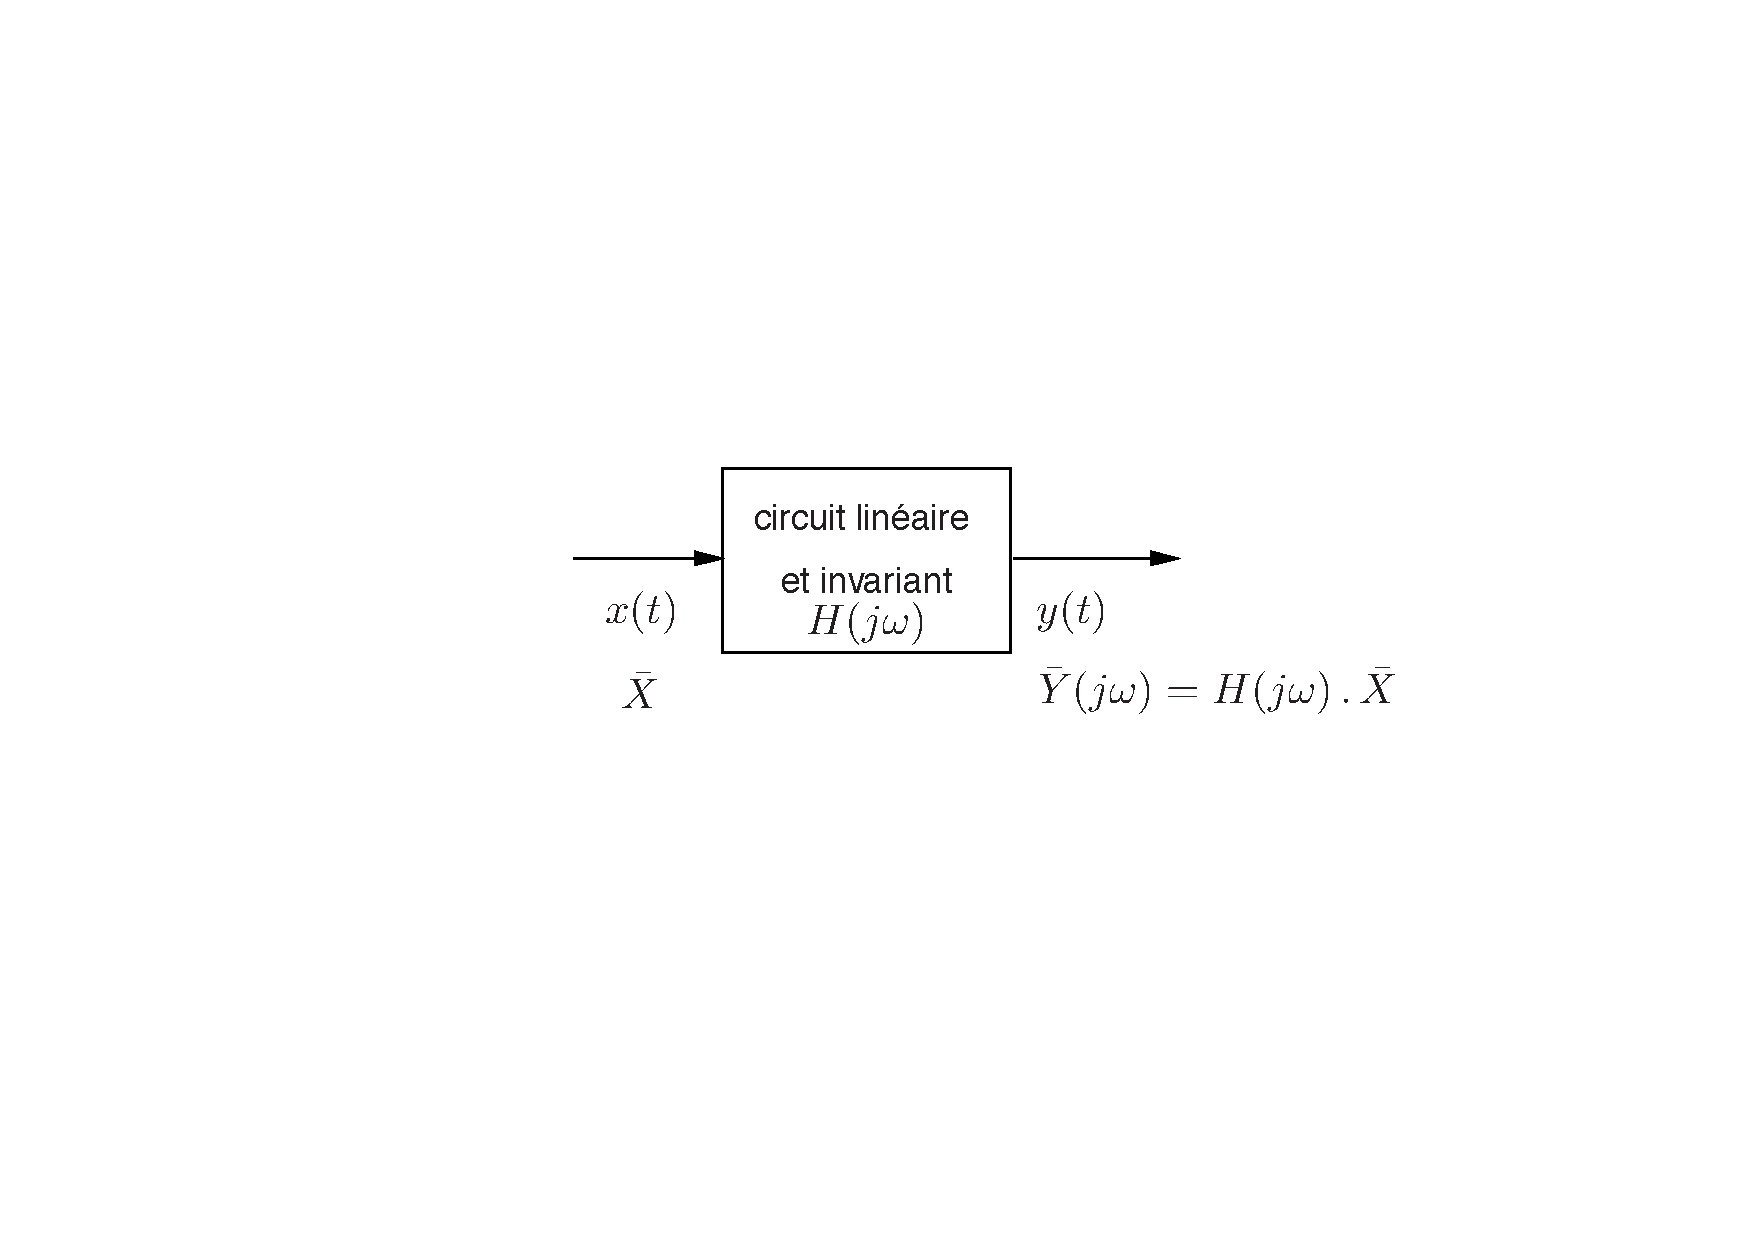
\includegraphics[width=0.6\linewidth]{figs/FR.pdf}
\end{center}
\[H(j\omega)=\frac{\bar{Y}(j\omega)}{\bar{X}}\]
	
\end{frame}

%--------------------------------------------------------------------------------
\begin{frame}{Exemple : impédance d'un circuit RL série}
Définissons l'entrée de notre système: $x(t)=i(t)=I_m \cos(\omega t+ \phi_i)$, ou en phaseurs $\bar{X}=\bar{I}=I_m  e^{j\phi_i}$, 
et la sortie $ \bar{Y}(j\omega)=\bar{U}=Z(j\omega)\bar{I}=(R+j\omega L)\bar{I}$.
\vspace{\baselineskip}

\begin{columns}
\begin{column}{0.45\textwidth}  
Dans ce cas la réponse fréquentielle se réduit à l'impédance du dipôle : 
\begin{gather*}
	H(j\omega)=\frac{\bar{Y}(j\omega)}{\bar{X}}=\frac{\bar{U}}{\bar{I}}=Z(j\omega)=R+j\omega L
\end{gather*}

\end{column}
\begin{column}{0.5\textwidth}
\begin{itemize}
	\item \alert{$|H(j\omega)|$}: réponse en amplitude, modifie l'\textbf{amplitude} du signal $x(t)$.
	\item \alert{$\angle H(j\omega)$}: réponse en phase,  modifie la \textbf{phase} du signal $x(t)$.
\end{itemize}
\end{column}
\vspace{\baselineskip}

\end{columns}
	Dans le domaine temporel : 
	\begin{align*}
		y(t)=u(t)& = \sqrt{R^2+\omega^2L^2}I_m \cos(\omega t +\phi_i+\arctan \frac{\omega L}{R})\\
		& = |H(j\omega)|I_m \cos(\omega t +\phi_i+\angle H(j\omega))
	\end{align*}
\end{frame}
%--------------------------------------------------------------------------------

\begin{frame}{Définition des 4 fonctions de transfert d'un quadripôle}
\begin{columns}
  \begin{column}{0.45\textwidth}
	\begin{center}
	\begin{circuitikz}[american voltages]% or tikzpicture
	\tikzset{quad/.style={draw, thick, minimum height=2.5cm, minimum width=2cm}}
	\node[quad] (A) at (0,0) {};
	\draw ($(A.north west)!.5!(A.west)$) node[right] {$1$} to[short, i<_=$\bar{I}_1$] ++(-.5,0) to[short,-*] ++(-0.2,0) coordinate (A1)
	($(A.south west)!.5!(A.west)$) node[right] {$1'$} to[short] ++(-.5,0) to[short,-*] ++(-0.2,0) coordinate (A1')
	($(A.north east)!.5!(A.east)$) node[left] {$2$} to[short, i<=$\bar{I}_2$] ++(.5,0) to[short,-*] ++(0.2,0) coordinate (A2)
	($(A.south east)!.5!(A.east)$) node[left] {$2'$} to[short] ++(.5,0) to[short,-*] ++(0.2,0) coordinate (A2');
	\draw (A1) to[open, v=$\bar{U}_1$] (A1');
	\draw (A2) to[open, v^=$\bar{U}_2$] (A2');
	\end{circuitikz}
	\end{center}
  \end{column}
  \begin{column}{0.45\textwidth}	
	\begin{align*}
		&H(j\omega)=\left.\frac{\bar{U}_2}{\bar{U}_1}\right|_{\bar{I}_2=0} \quad \text{gain en tension}\\
		&H(j\omega)=\left.\frac{\bar{I}_2}{\bar{I}_1}\right|_{\bar{U}_2=0}\quad \text{gain en courant}\\
		&H(j\omega)=\left.\frac{\bar{U}_2}{\bar{I}_1}\right|_{\bar{I}_2=0} \quad \text{impédance de transfert}\\
		&H(j\omega)=\left.\frac{\bar{I}_2}{\bar{U}_1}\right|_{\bar{U}_2=0} \quad \text{admittance de transfert}
	\end{align*}
\end{column}
\end{columns}
	
\end{frame}
%--------------------------------------------------------------------------------

\begin{frame}{Forme analytique, pôles et zéros}
	
	Toute réponse fréquentielle d'un circuit peut se mettre sous la \alert{forme rationnelle} $\boxed{H(j\omega)=\frac{N(j\omega)}{D(j\omega)}}$
	où $N(j\omega)$ et $D(j\omega)$ sont deux \alert{polynomes} en $j\omega$ à coefficients réels.
	
	Les racines de 
	\begin{itemize}
		\item $D(j\omega)=0$ sont les \alert{pôles} de la fonction. Ils correspondent aux fréquences naturelles du circuit.
		\item $N(j\omega)=0$ sont les \alert{zéros} de la fonction. \`A ces fréquences :
		\[H(j\omega)=0 \quad \rightarrow \quad Y(j\omega)=0 \quad \rightarrow \quad \text{Elimination de cette fréquence }\]
	\end{itemize}
	
	
	
	
	
	Pour éviter des calculs en nombres complexes, il est courant de remplacer la variable $j\omega$ par $s$ (formalisme de Laplace, cf. cours de signaux et systèmes).
	La fonction 
	\[H(s)=H(j\omega)|_{j\omega=s}\]
	est alors appelée {\bf fonction de transfert}.
\end{frame}
%--------------------------------------------------------------------------------
\begin{frame}{Exemple : quadripôle RC}
	
\begin{columns}
	\begin{column}{0.4 \linewidth}
		\begin{center}
			\begin{circuitikz}[american voltages]% or tikzpicture
				\draw (0,0) coordinate (A1)
				to[short, *-*] ++(2,0) coordinate (C)
				to[short, *-*] ++(1,0) coordinate (A2);
				\draw (0,2) coordinate (A1')
				to[R, *-*, l=$R$] ++(2,0) coordinate (C')
				to[short, *-*] ++(1,0) coordinate (A2');
				\draw (C) to[C, l_=$C$] (C');
				\draw (A1') to[open, v=$\bar{U}_1$] (A1);
				\draw (A2') to[open, v^=$\bar{U}_2$] (A2);
			\end{circuitikz}
		\end{center}
	\end{column}
	\begin{column}{0.6 \linewidth}
	Réponse fréquentielle gain en tension :
	\[H(j\omega)=\left.\frac{\bar{U}_2}{\bar{U}_1}\right|_{\bar{I}_2=0}=
	\frac{1/j\omega C}{R+1/j\omega C}=\frac{1}{1+j\omega RC}\]
	
	Fonction de transfert :
	\[H(s)=\frac{1}{1+sRC}\]

	\end{column}
\end{columns}
\vfill
\begin{itemize}
	\item zéro : $\quad j\omega = s  \rightarrow \infty \qquad |H(j\omega)|\rightarrow 0 \text{~pour~~} \omega \rightarrow \infty$
	\item pôle : $\quad j\omega=s= -\frac{1}{RC} \qquad \text{= fréquence naturelle}$
\end{itemize}
	
\end{frame}
%--------------------------------------------------------------------------------
\begin{frame}{Représentation de $H(j\omega)$}
	
Soit $\omega_0=\frac{1}{RC}$
\begin{columns}
\begin{column}{0.48 \linewidth}
	$$H =|H(j\omega)| =\frac{1}{\sqrt{1+(\omega RC)^2}} =\frac{1}{\sqrt{1+(\omega/\omega_0)^2}}$$
\end{column}
\begin{column}{0.48 \linewidth}
	$$\angle H(j\omega) =-\arctan \frac{\omega}{\omega_0}$$
\end{column}
\end{columns}
\begin{center}
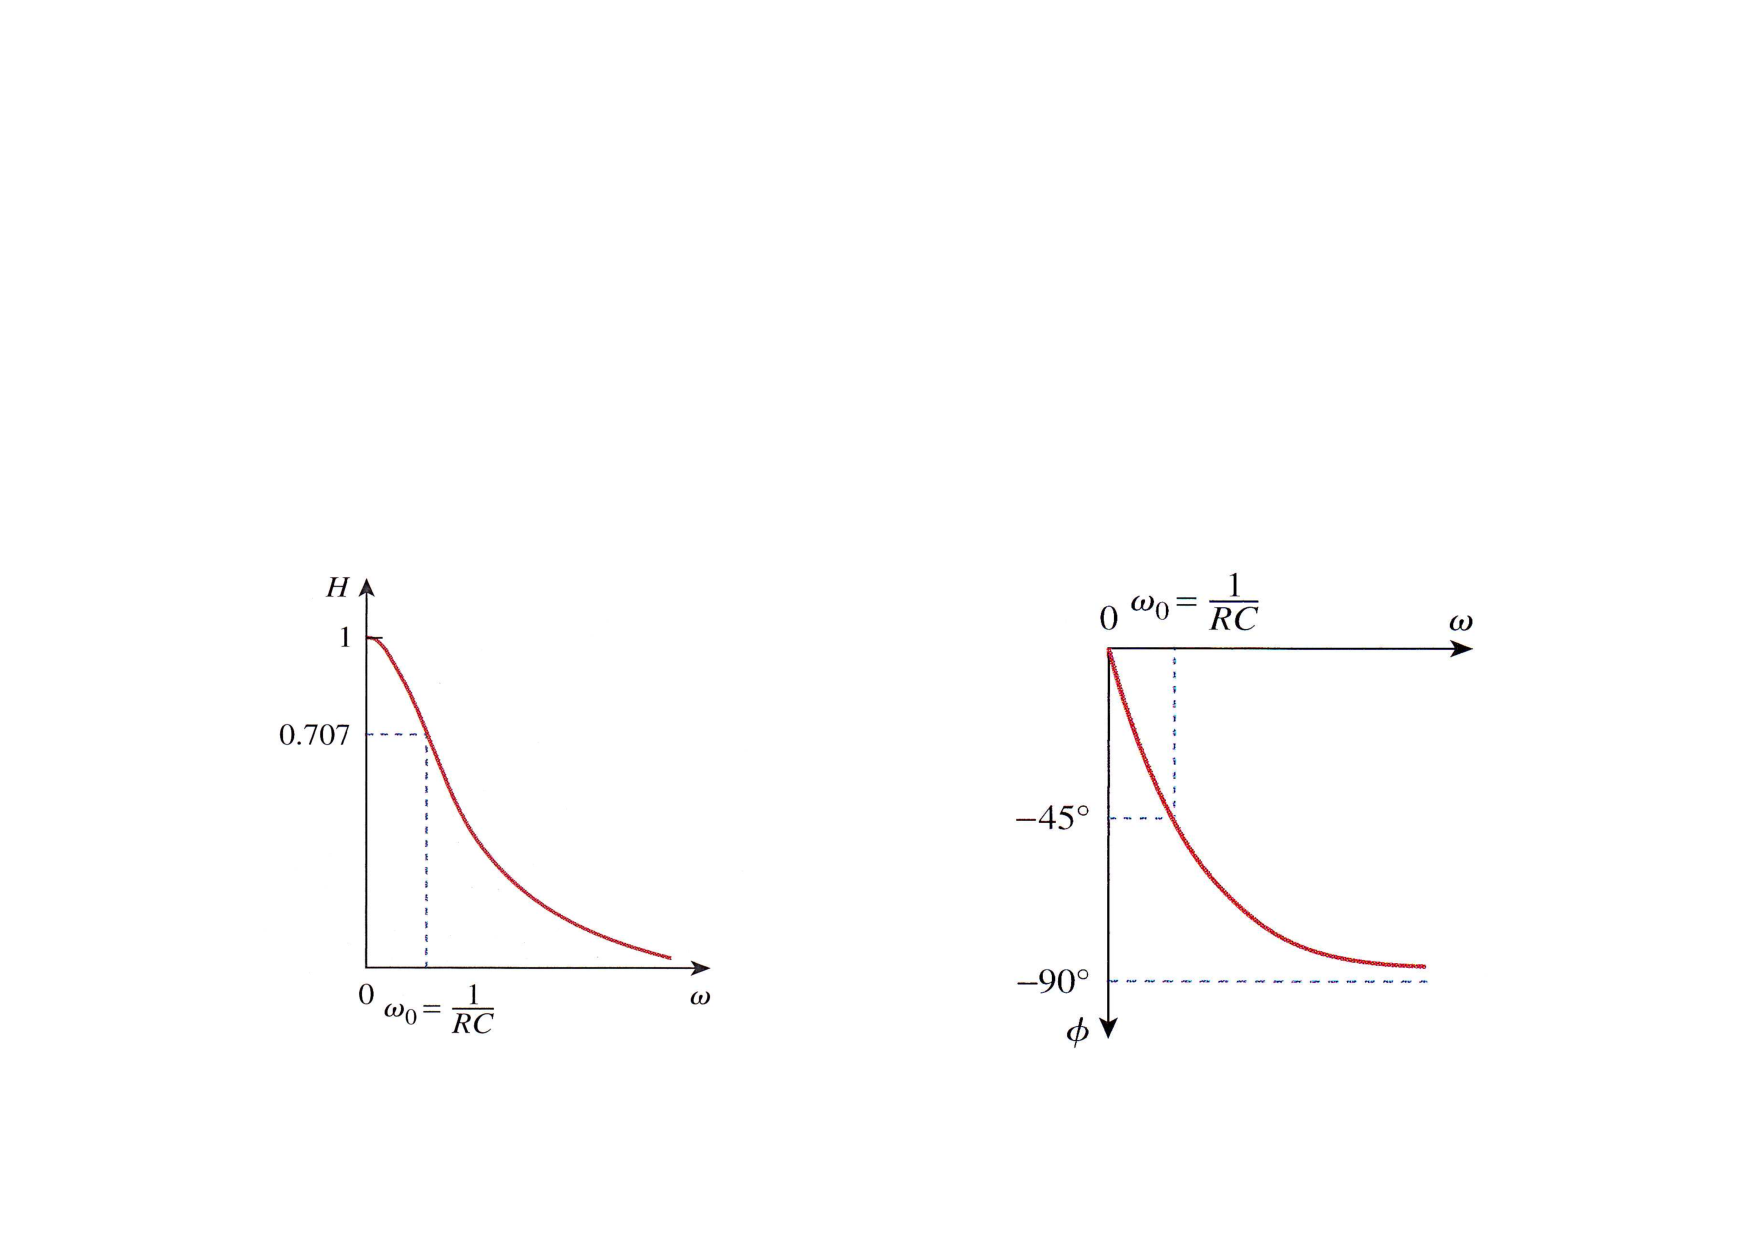
\includegraphics[width=0.6\linewidth]{figs/filtre_RC}
\end{center}
\begin{columns}
\begin{column}{0.48 \linewidth}
$|H(j\omega_0)|=\frac{1}{\sqrt{2}}=0.707$
\end{column}
\begin{column}{0.48 \linewidth}
$\phi_0=\angle H(j\omega_0)=-\frac{\pi}{4}$
\end{column}
\end{columns}
\end{frame}
%--------------------------------------------------------------------------------
\begin{frame}{Le décibel ou dB}
	\begin{columns}
  \begin{column}{0.45\textwidth}  
	\begin{block}{Le décibel}
	Échelle logarithmique de mesure du rapport entre deux  puissances, ou gain en puissance 
	\[G_{dB}=10\log_{10}\frac{P_2}{P_1}\]
	\end{block}
  \end{column}
  \begin{column}{0.45\textwidth}
	Si l'on exprime ce gain \textbf{en fonction de $U$ ou $I$}, 
	on obtient :
	\[P \propto U^2, I^2 \quad \Rightarrow G_{dB}=\mathbf{20}\log_{10}\frac{U_2}{U_1}= \mathbf{20}\log_{10}\frac{I_2}{I_1}\]
  \end{column}
\end{columns}

	
	
	Valeurs caractéristiques :
	\begin{center}
		\begin{tabular}{ll|c}
			&& $G_{dB}$\\ \hline
			$P_1=P_2$ &  $U_1=U_2$ & 0\\
			$P_2=\frac{1}{2}P_1$ & $U_2=\frac{1}{\sqrt{2}}U_1$  & -3\\
			$P_2=\frac{1}{10}P_1$ & $U_2=\frac{1}{\sqrt{10}}U_1$  & -10\\ \hline
		\end{tabular} \hspace*{1cm}
		\begin{minipage}[c]{0.35\linewidth}
			Dans l'exemple précédent, pour $\omega=\omega_0$
			\[\mathbf{20} \log_{10}\frac{|H(\omega_0)|}{|H(0)|}=-3 \, \text{dB}\]
		\end{minipage}
	\end{center}
	
	
\end{frame}
%--------------------------------------------------------------------------------

\subsection{Exemples de filtres}
\begin{frame}{Définition}
	
	\begin{block}{Filtre}
		Circuit qui permet d'éliminer ou atténuer fortement certaines
		fréquences d'un signal tout en affectant le moins possible les autres fréquences.
	\end{block}

	Un filtre de réponse fréquentielle idéale est impossible à réaliser en
	pratique.
	
	\begin{block}{Pulsation de coupure à -3 dB}
	On définit la pulsation de coupure à -3 dB qui limite la bande passante:
	\[\omega_c~~ \text{telle que} \quad |H(\omega_c)|=\frac{1}{\sqrt{2}}\]
	\end{block}
\end{frame}	
\begin{frame}{Catégories de filtres et réponses fréquentielles idéales}
	\begin{center}
	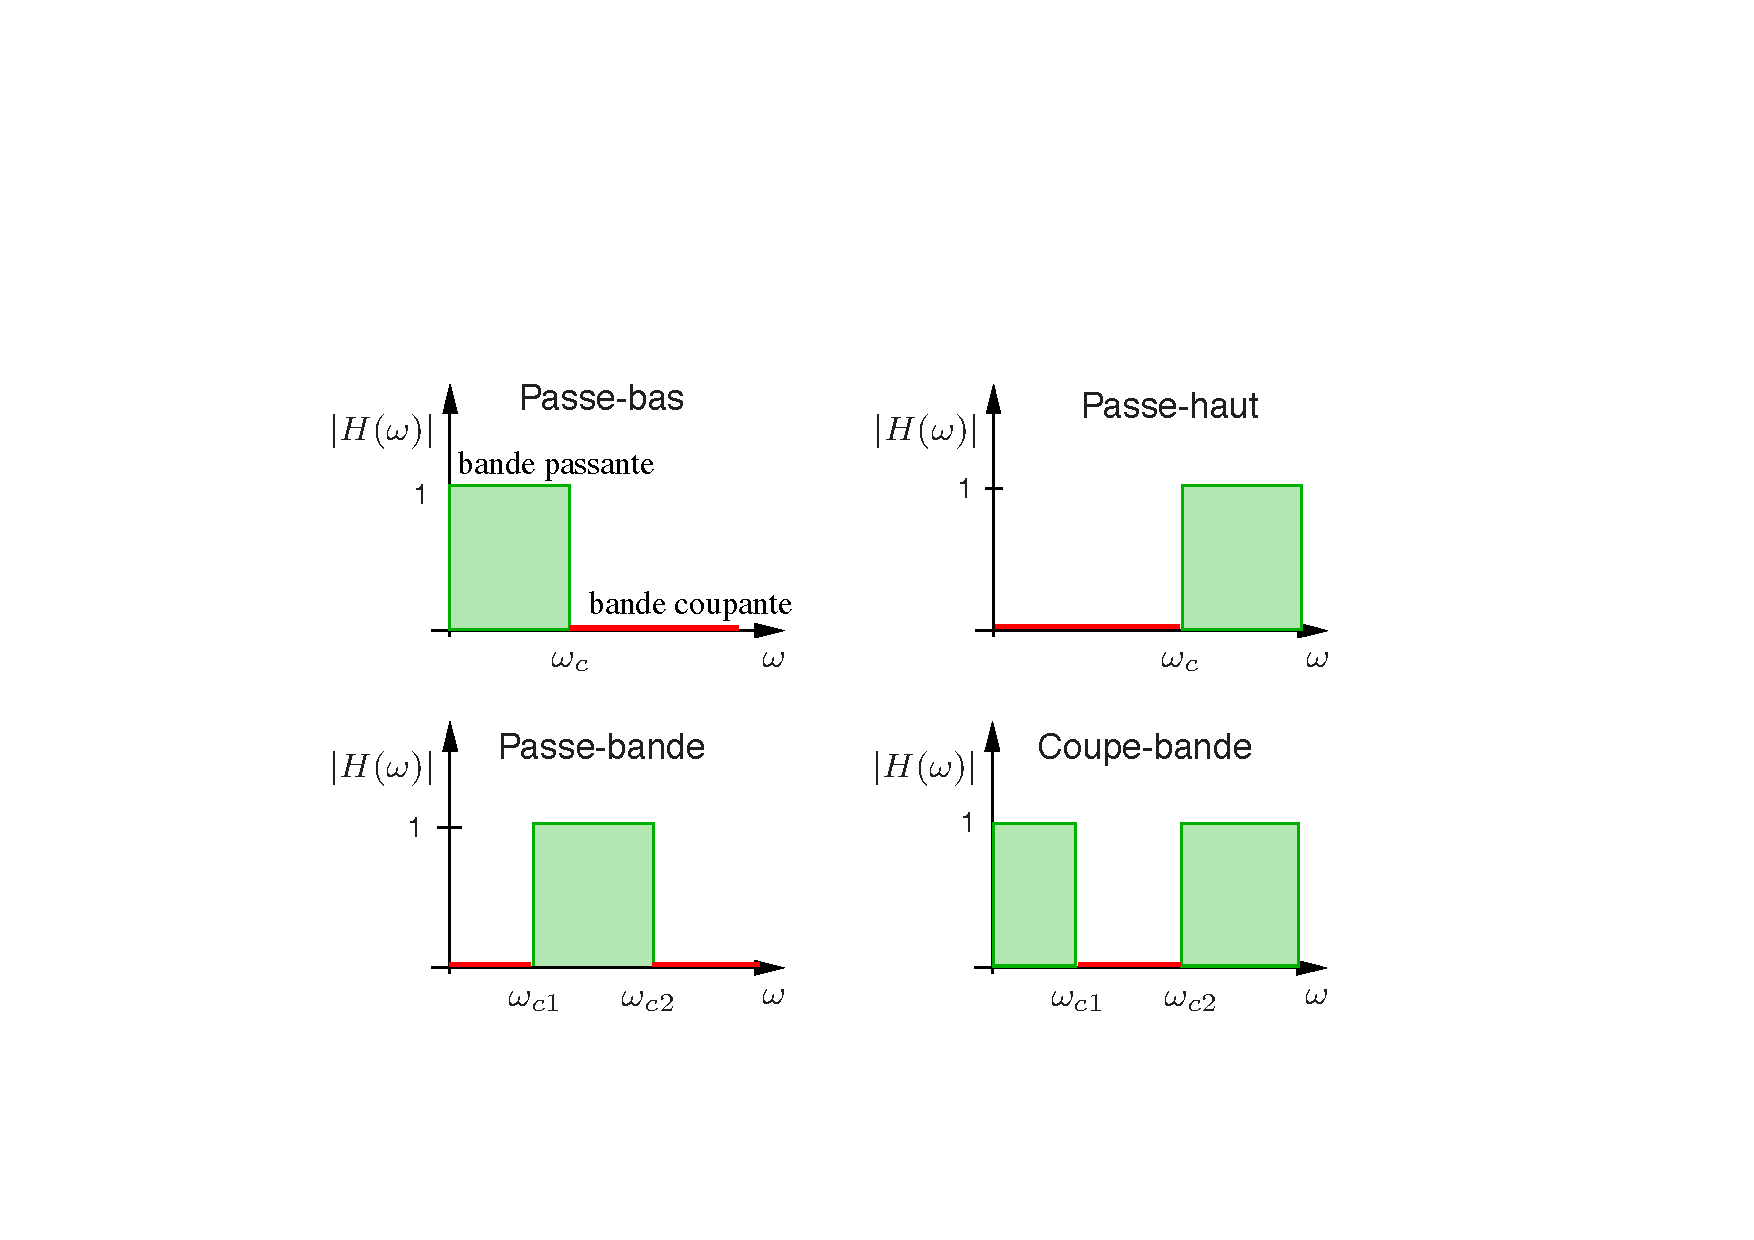
\includegraphics[width=0.6\linewidth]{figs/filtres}
	\end{center}
	\vspace*{-3mm}
	$\omega_c$ : pulsation de coupure
\end{frame}
%--------------------------------------------------------------------------------
\begin{frame}{Exemple de filtre  passe-bas du 1er ordre}
	
	\begin{minipage}[c]{0.4\linewidth}
		\begin{center}
		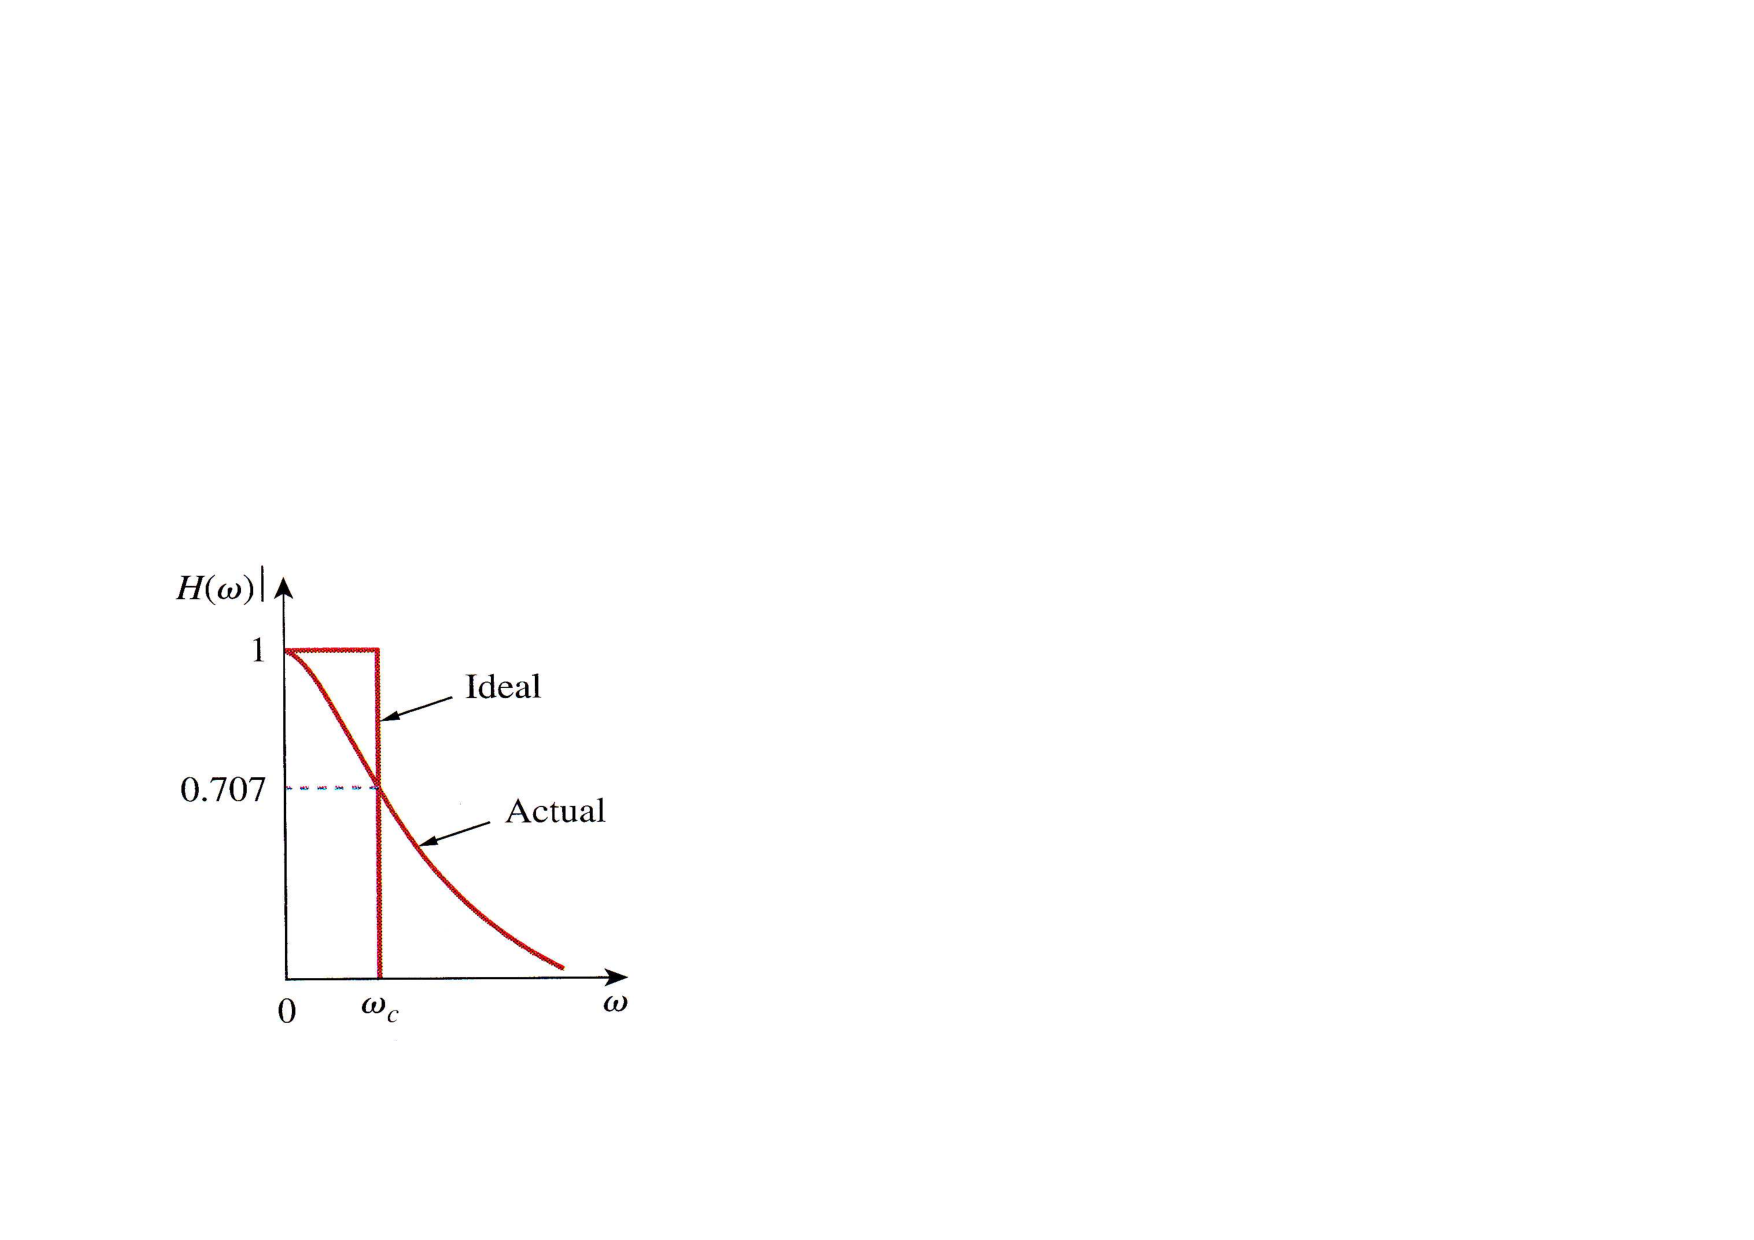
\includegraphics[width=0.7\linewidth]{figs/filtre_PB_ordre1}
		\end{center}
	\end{minipage}
	\begin{minipage}[c]{0.55\linewidth}
		\centering
			\begin{circuitikz}[american voltages, scale=0.9]% or tikzpicture
				\ctikzset{bipoles/length=0.5cm}
				\draw (0,0) coordinate (A1)
				to[short, *-*] ++(2,0) coordinate (C)
				to[short, *-*] ++(1,0) coordinate (A2);
				\draw (0,2) coordinate (A1')
				to[R, *-*, l=$R$] ++(2,0) coordinate (C')
				to[short, *-*] ++(1,0) coordinate (A2');
				\draw (C) to[C, l_=$C$] (C');
				\draw (A1') to[open, v=$\bar{U}_1$] (A1);
				\draw (A2') to[open, v^=$\bar{U}_2$] (A2);
			\end{circuitikz} \\[5mm]
			$H(j\omega) = \frac{\bar{U}_2}{\bar{U}_1} = \frac{1}{1+j\omega R C}$
	\end{minipage}
	\vfill 
	Pulsation de coupure à -3 dB~:			$\omega_c=\frac{1}{RC}=\omega_0$
			
	\everycircuitlink{https://everycircuit.com/circuit/5002680858705920}
\end{frame}
%--------------------------------------------------------------------------------
\begin{frame}{Exemple de filtre passe-haut du 1er ordre}
	
	\begin{minipage}[c]{0.4\linewidth}
		\begin{center}
			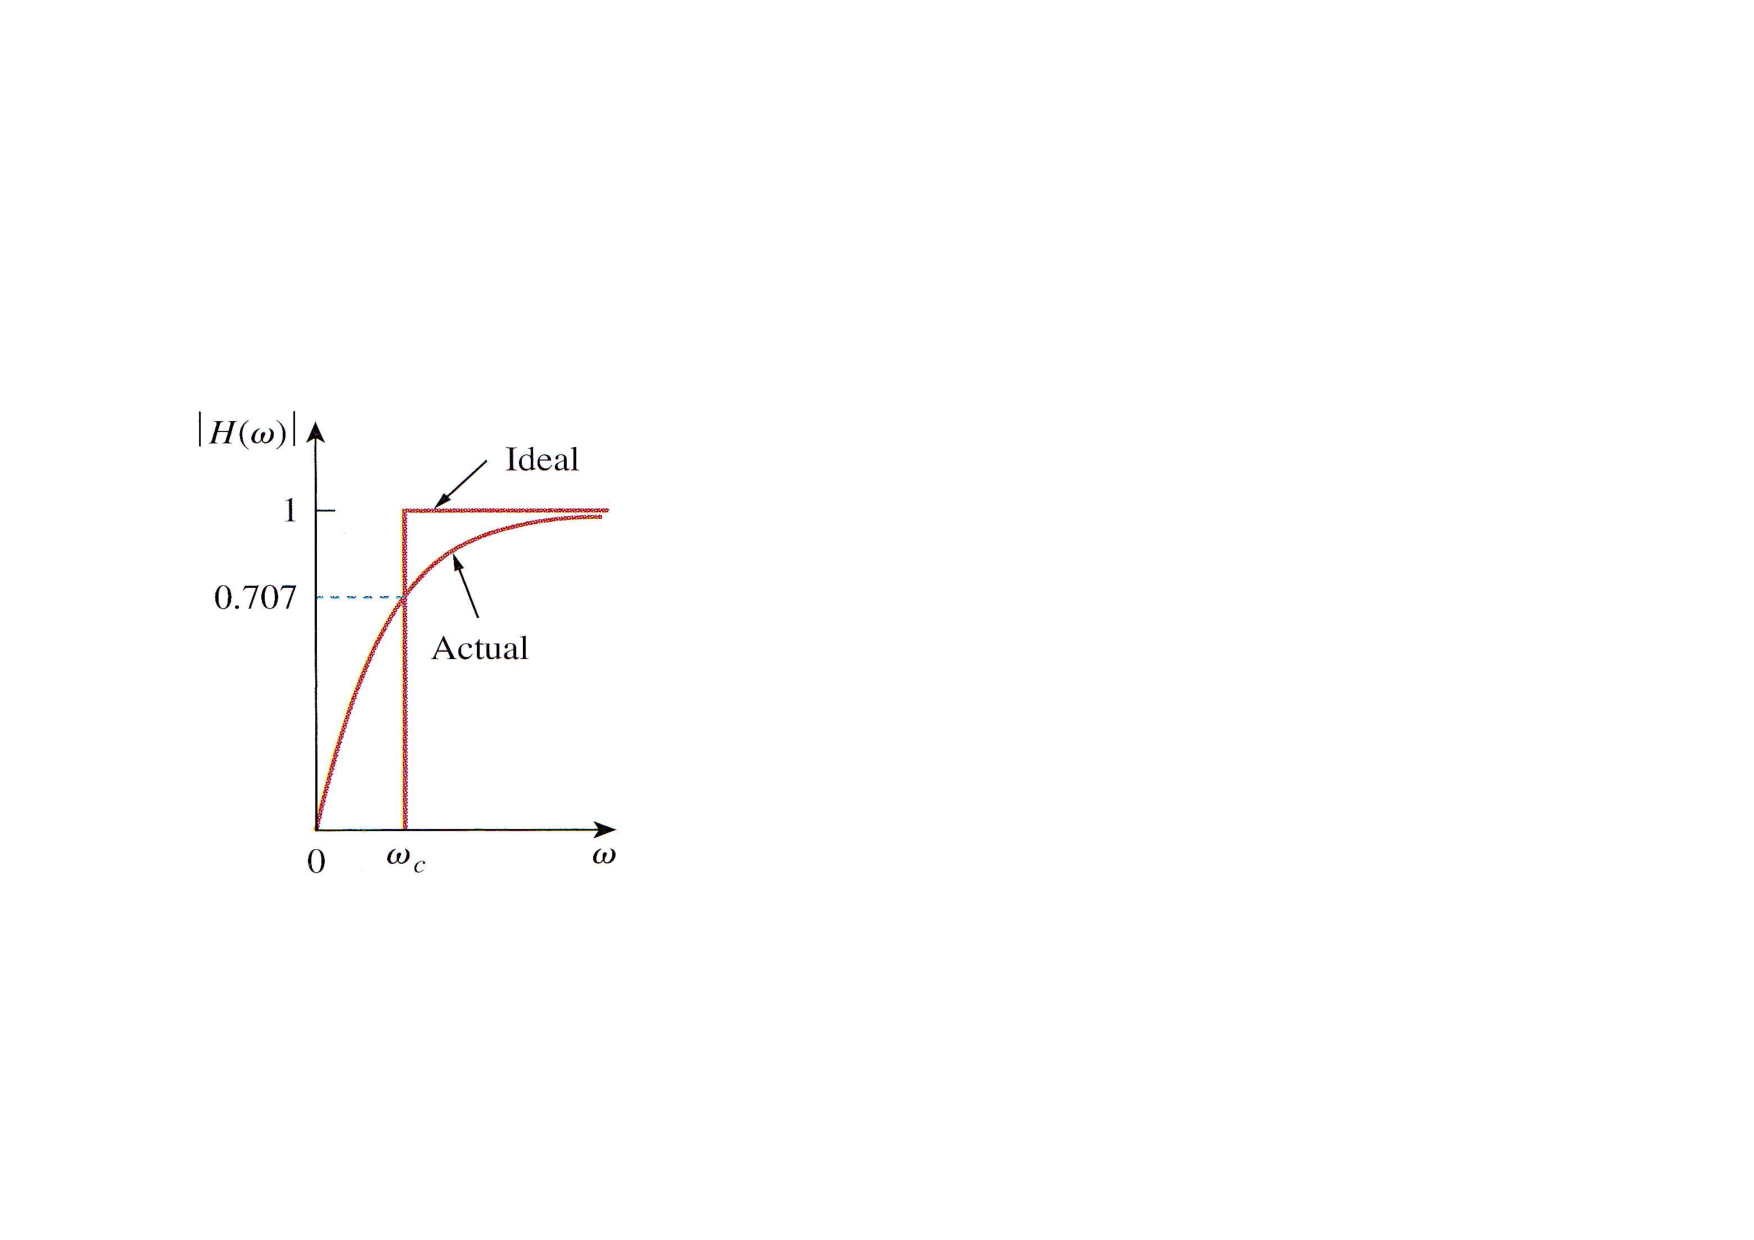
\includegraphics[width=0.7\linewidth]{figs/filtre_PH_ordre1}
		\end{center}
	\end{minipage}
	\begin{minipage}[c]{0.55\linewidth}
		\centering 
		\begin{circuitikz}[american voltages, scale=0.9]% or tikzpicture
			\ctikzset{bipoles/length=0.5cm}
			\draw (0,0) coordinate (A1)
			to[short, *-*] ++(2,0) coordinate (C)
			to[short, *-*] ++(1,0) coordinate (A2);
			\draw (0,2) coordinate (A1')
			to[C, *-*, l=$C$] ++(2,0) coordinate (C')
			to[short, *-*] ++(1,0) coordinate (A2');
			\draw (C) to[R, l_=$R$] (C');
			\draw (A1') to[open, v=$\bar{U}_1$] (A1);
			\draw (A2') to[open, v^=$\bar{U}_2$] (A2);
		\end{circuitikz}\\[5mm]
		$H(j\omega) = \frac{\bar{U}_2}{\bar{U}_1} = \frac{j\omega R C}{1+j\omega R C}$
		
	\end{minipage}
	\vfill 
	Pulsation de coupure à -3 dB~: $\omega_c=\frac{1}{RC}$
	
	\everycircuitlink{https://everycircuit.com/circuit/5419822108246016}

\end{frame}

%--------------------------------------------------------------------------------

\section{L'amplificateur opérationnel}

\begin{frame}{Questions}

\begin{itemize}
	\item Connaissez-vous une manière d'amplifier un signal (tension ou courant) ?
	\item Connaissez-vous une manière de réaliser des opérations mathématiques sur des signaux (addition, division, dérivation, ...) ?
	\item Peut-on amplifier uniquement une partie d'un signal?
\end{itemize}

\everycircuitlink{https://everycircuit.com/circuit/4810317695680512}

\end{frame}


\begin{frame}{L'élément amplificateur opérationnel}
	
	
	Composant électronique introduit dans les années 60 (calculateur analogique).
	
	En théorie des circuits, on ne s'intéresse pas à sa constitution
	interne mais à son fonctionnement, observé d'un certain nombre de ses
	bornes :
	\vspace{\baselineskip}
	\begin{columns}
		\begin{column}{0.5\linewidth}

			\begin{center}
				
				\begin{circuitikz} 
					\draw
					(0,0) node[op amp] (opamp) {}
					(opamp.+) node[left] {$v_p$}
					(opamp.-) node[left] {$v_n$}
					(opamp.out) node[right] {$v_o$}
					(opamp.up) --++(0,0.5) node[above]{$+V_{cc}$}
					(opamp.down) --++(0,-0.5) node[below]{$-V_{cc}$}
					;
				\end{circuitikz}
			\end{center}
		\end{column}
		\begin{column}{0.5\linewidth}
			\begin{itemize}
				\item entrée inverseuse ($v_n$)
				\item entrée non inverseuse ($v_p$)
				\item sortie ($v_o$)
				\item alimentation positive ($+V_{cc}$)
				\item alimentation négative ($-V_{cc}$)
			\end{itemize}
		\end{column}
	\end{columns}
	\vfill
	Par la suite, \alert{AO} $=$ amplificateur opérationnel.
\end{frame}


%--------------------------------------------------------------------------------

\begin{frame}{}
	\begin{center}
		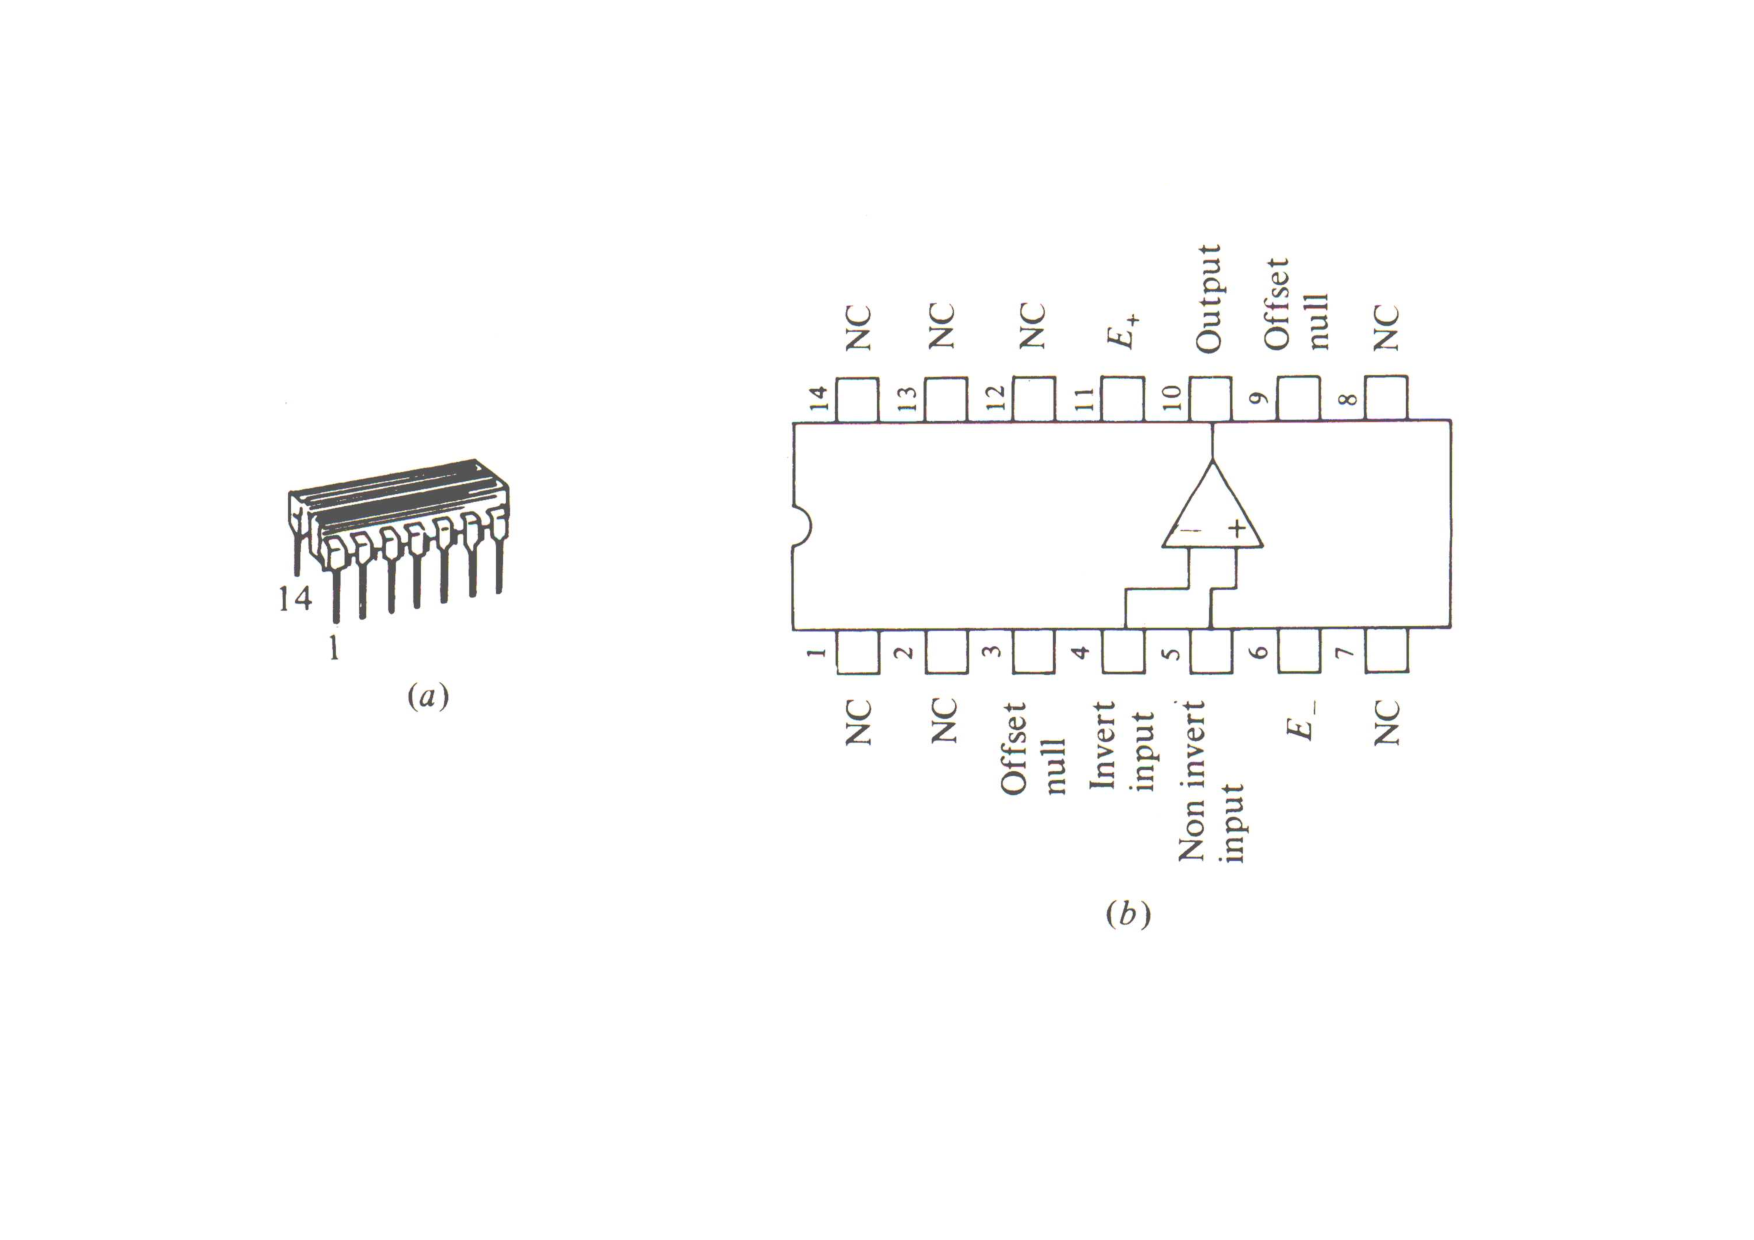
\includegraphics[width=0.9\linewidth]{figs/AO_3}
	\end{center}
\end{frame}


\subsection{Caractéristiques de fonctionnement}
\begin{frame}{Caractéristiques de fonctionnement}
	\begin{center}
		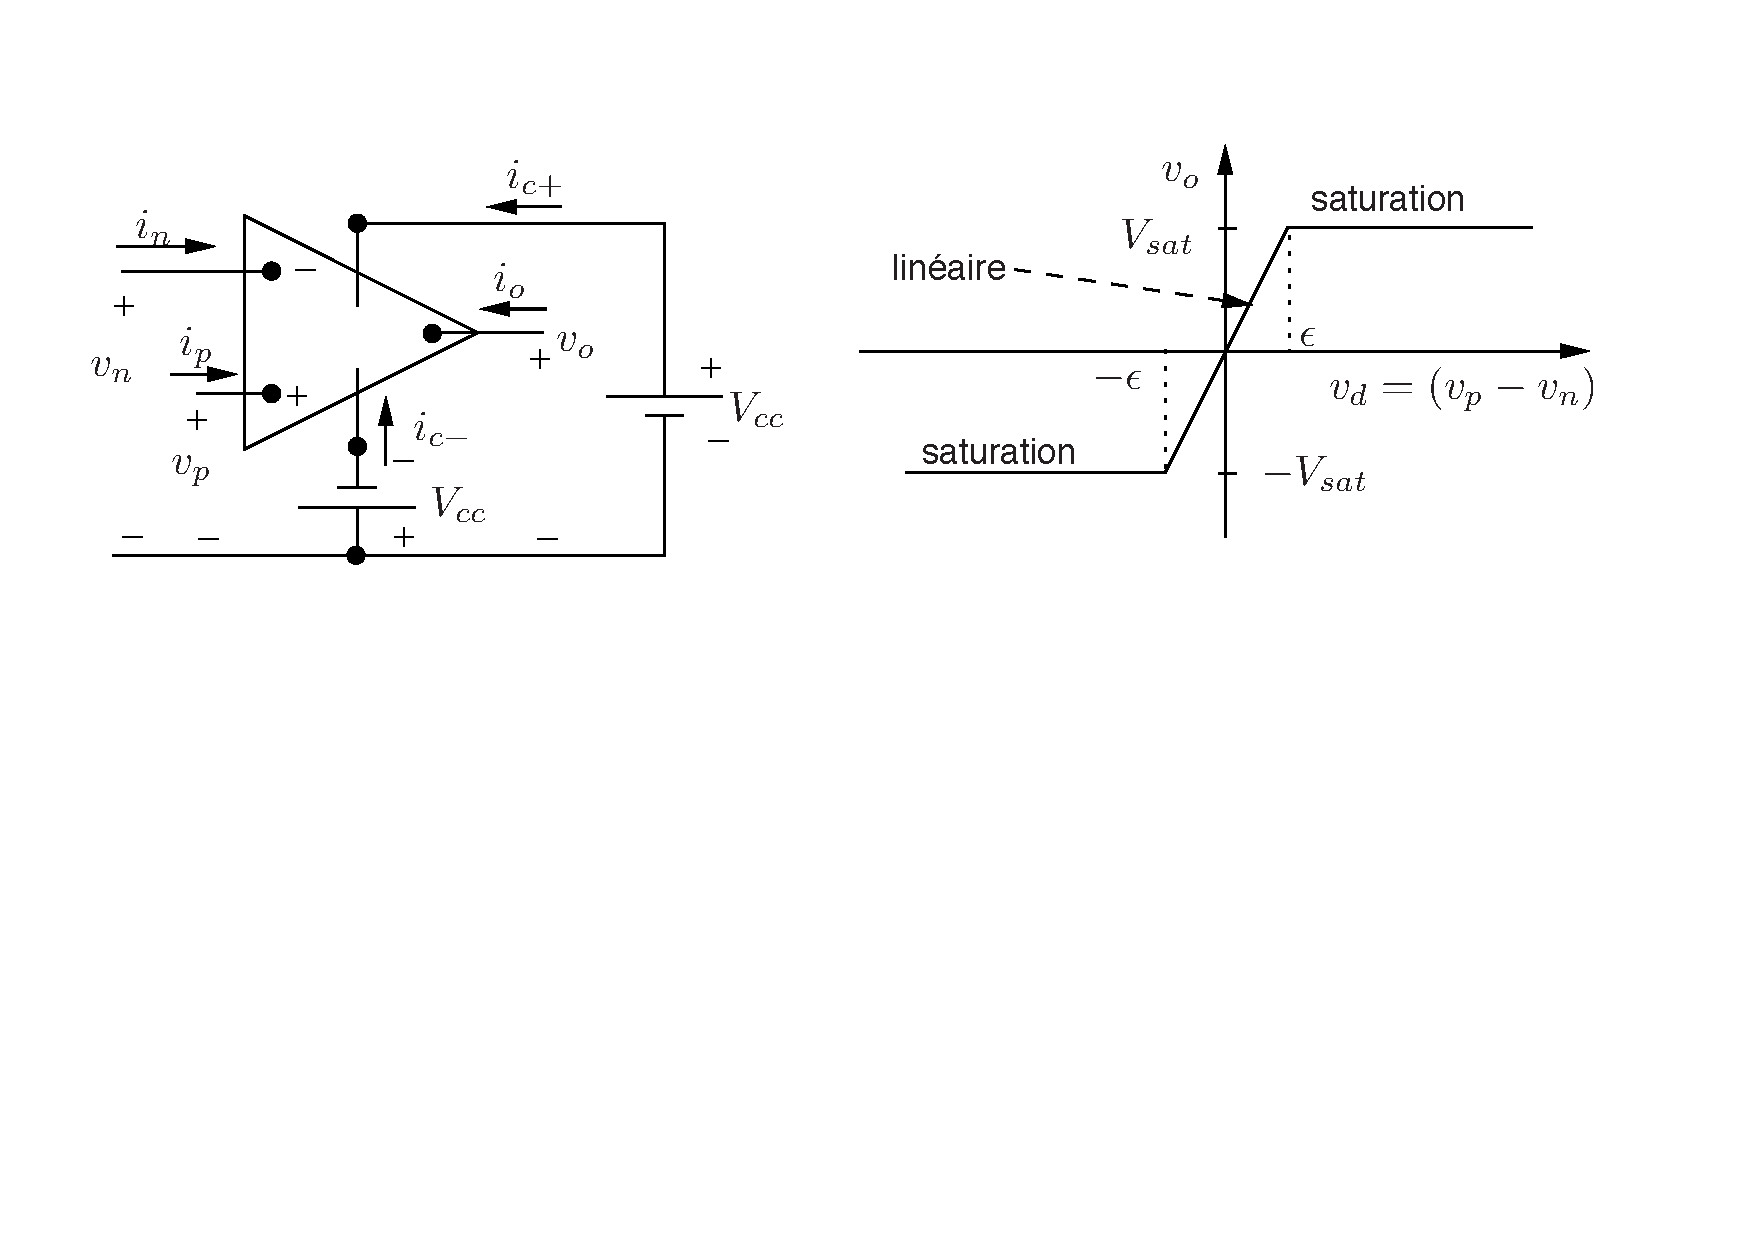
\includegraphics[width=0.8\linewidth]{figs/AO_caracteristique}
	\end{center}
	\begin{columns}
  \begin{column}{0.6\textwidth}  
	Avec $v_d = v_p-v_n$ et $\epsilon = \frac{V_{sat}}{\textcolor{blue}{A}}$, l'AO fonctionne \textbf{dans la plage linéaire} si  \alert{$v_d \in [-\epsilon,\epsilon]$}, au-delà,
	 en \textbf{saturation} : 
	\vspace*{-1ex}
	\[v_o=\begin{cases}
	-V_{sat} & v_d <  -\epsilon\\
	\textcolor{blue}{A}v_d & -\epsilon \leq v_d \leq \epsilon \\
	+V_{sat}& v_d> \epsilon
	\end{cases}\]
  \end{column}
  \begin{column}{0.4\textwidth}
	Notez que dans le cas ci-dessus, $$V_{sat} = V_{cc}.$$
	
	\vfill
	Équation pour les courants :	$$i_p+i_n+i_o+\underbrace{i_{c+}+i_{c-}}_{\text{Alimentation !}}=0$$
  \end{column}
\end{columns}

\end{frame}

\begin{frame}{Comment pourrait-on faire la même chose que dans l'expérience précédente avec une source commandée ?}

	Donc en remplaçant l'amplificateur opérationnel.

	\everycircuitlink{https://everycircuit.com/circuit/6475814073925632}

	

\end{frame}

\begin{frame}{Réponse}
On notera que l'amplificateur peut être approximé comme à la figure suivante  \textbf{dans sa plage de fonctionnement linéaire} :
\begin{center}
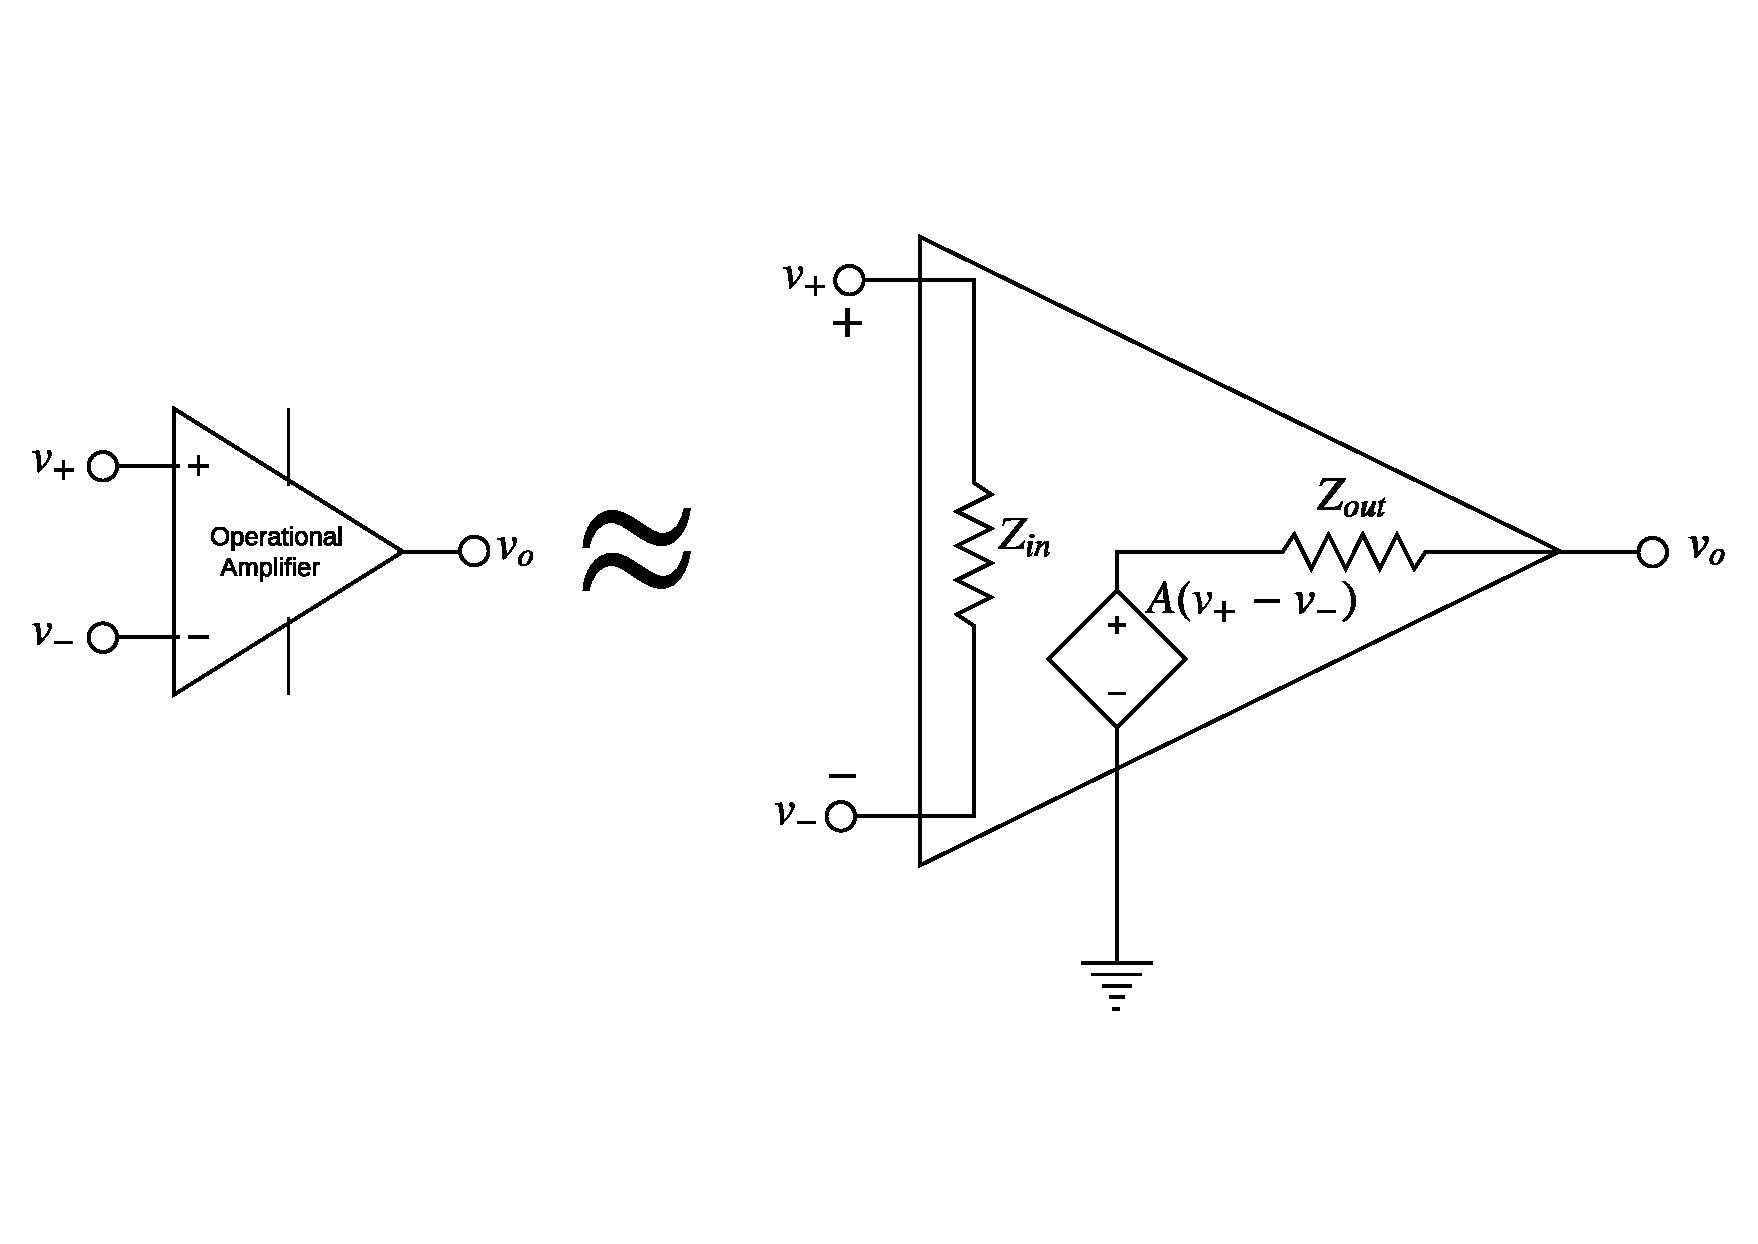
\includegraphics[width=0.6\linewidth]{figs/OpAmpEquivalent}
\end{center}
\vfill

On peut cependant obtenir un modèle idéal encore plus simple en faisant quelques \textbf{hypothèses}.
\end{frame}



%-------------------------------------------------------------------

\subsection{Modèle idéal}
\begin{frame}{Modèle idéal}
	
	\begin{block}{Valeurs typiques des paramètres d'un AO en pratique}
		\begin{itemize}
			\item $V_{sat} < 20$ V
			\item $A$ de l'ordre de $10^4$ à $10^5$
			\item $\rightarrow$ dans la plage de fonctionnement linéaire
			$|v_p-v_n|< 2$ mV
			\item $i_p$, $i_n$ de l'ordre de 0.1 mA
		\end{itemize}
	\end{block}
	
	\begin{block}{Modèle idéal}
		\begin{itemize}
			\item $A=\infty \rightarrow \epsilon=0$ et $v_p=v_n$
			\item $i_p=i_n=0 \rightarrow Z_{in}=\infty$
		\end{itemize}
	\end{block}
	
\end{frame}

%-------------------------------------------------------------------

\begin{frame}{Modèle idéal ...}
	\begin{center}
		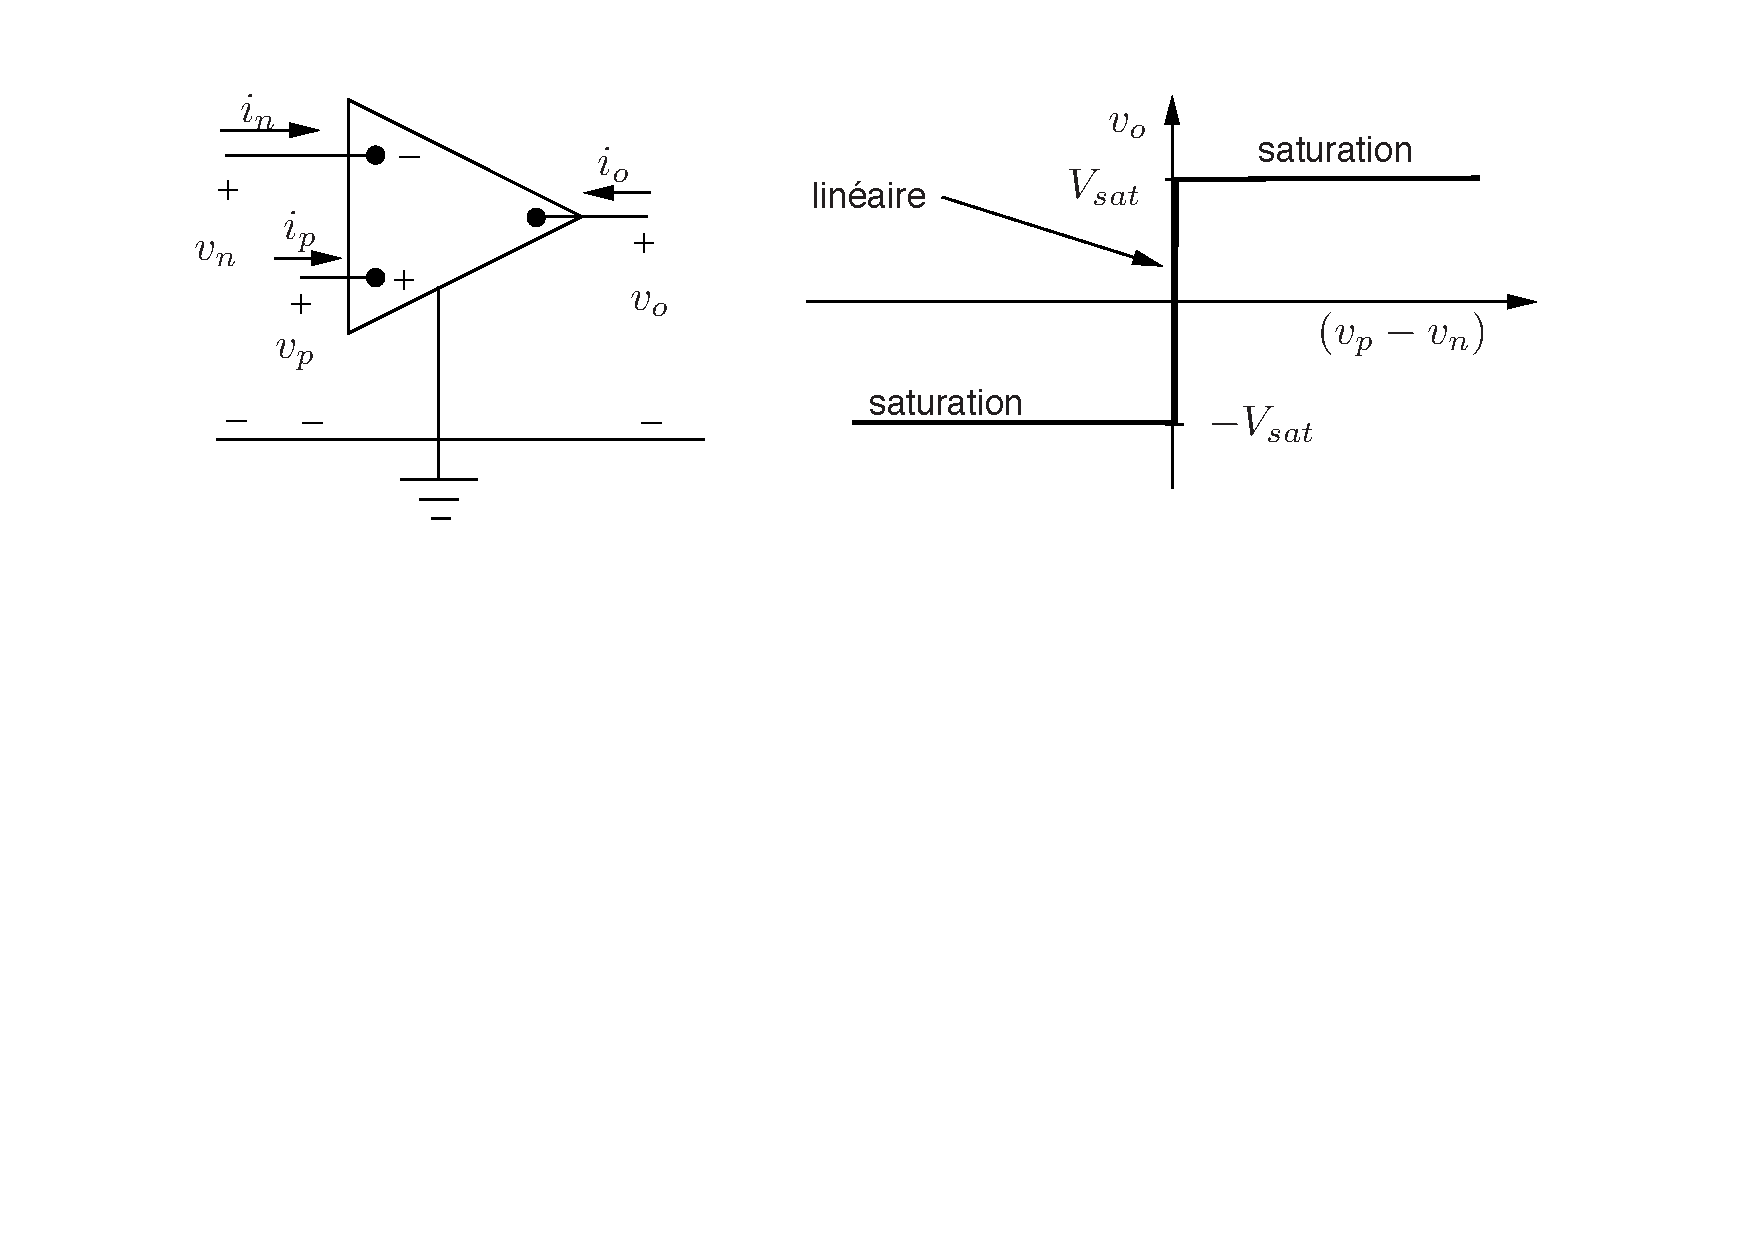
\includegraphics[width=0.9\linewidth]{figs/AO}
	\end{center}
	\begin{eqnarray*}
		i_n & = & 0 = i_p \\
		v_d & =& 0 \quad \text{si~} -V_{sat} < v_o < V_{sat}\\
%s		v_o &= &V_{sat}\frac{|v_d|}{v_d} \quad \text{si~} v_d \neq 0
	\end{eqnarray*}
	Remarques importantes : 
	\begin{itemize}
		\item \textbf{En mode de fonctionnement linéaire, $v_o$ est fixé par le circuit
			extérieur à l'AO} : présence d'une contre-réaction négative.
		\item \alert{Attention : $i_o\neq 0$} car courant débité par les
		sources d'alimentation
		\item comme nous supposons être dans la plage linéaire, nous omettons d'indiquer les entrées d'alimentation. Cependant, il faut toujours vérifier que les hypothèses sont vérifiées.
	\end{itemize}
\end{frame}

\begin{frame}{Contre réaction}
La \textit{contre-réaction}, plus communément appelée \textit{feedback}, provient du circuit qui ramène à l'entrée une fraction du signal de sortie : 

\begin{columns}
\begin{column}{0.4\textwidth}
\begin{center}
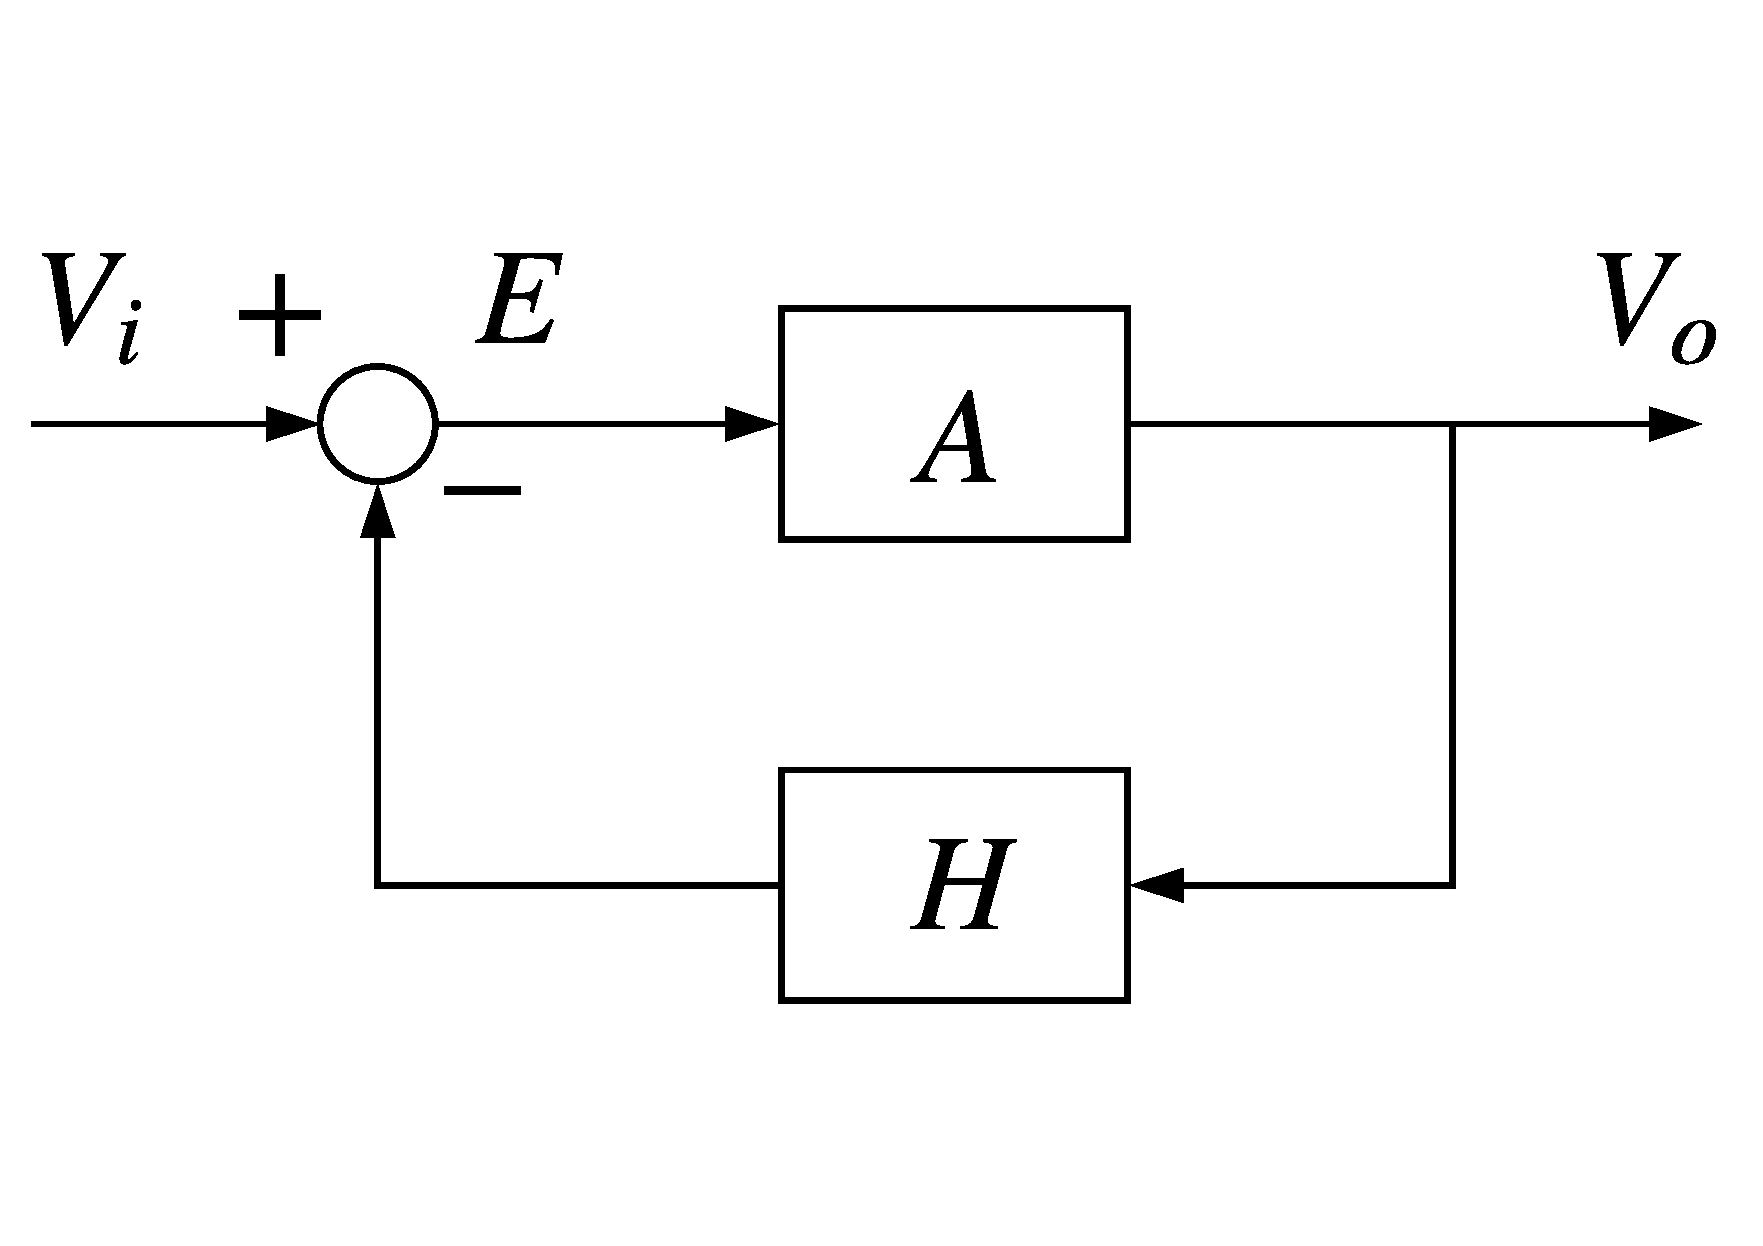
\includegraphics[width=0.7\textwidth]{figs/feedback}
\end{center}
\end{column}\hfill
\begin{column}{0.6\textwidth}
$E$ est le signal différentiel, $A$ le gain de la boucle directe, $H$ le gain de la boucle de retour ou de contre-réaction.
\end{column}
\end{columns}\vspace{2mm}

\begin{columns}
  \begin{column}{0.6\textwidth}
	Le gain global "en boucle fermée" du système se déduit comme suit :
	$E = V_i- HV_o$, $V_o = AE$, donc $V_o = AV_i -AHV_o$.
	Ou encore 
	\begin{equation}\label{eq:feedback_1}
	\frac{V_o}{V_i} = \frac{A}{1+AH} = \frac{1}{1/A+H}.
	\end{equation}
  \end{column}
  \begin{column}{0.4\textwidth}
	Pour un gain $A$ infini (cas de l'AO idéal), l'expression (\ref{eq:feedback_1}) devient :
	\begin{equation}
	\frac{V_o}{V_i} = \frac{1}{H}.
	\end{equation}
  \end{column}
\end{columns}

\textbf{Ceci montre comment, grâce à la contre-réaction, il est possible d'obtenir une tension de sortie finie avec un élément de gain infini.}
\end{frame}

\begin{frame}{Dans la suite de cette leçon ...}
Nous allons considérer quelques montages d'AO avec boucle de feedback et les caractériser.

\vfill

Nous faisons toujours l'hypothèse de l'AO idéal.
\end{frame}

%-------------------------------------------------------------------
\section{Le montage amplificateur inverseur}
\subsection{Caractéristiques}
\begin{frame}{Gain en tension}
	
	
	\begin{columns}
		\begin{column}{0.5\linewidth}
			On cherche à déterminer le gain en tension $\frac{v_o}{v_s}$ du montage. \vfill 
			\begin{circuitikz} [scale=0.9]
				\draw (3.5,1.5) node[op amp] (opamp) {} % Opamp
				(opamp.+) node[left] {$v_p$}
				(opamp.-) node[below] {$v_n$};
				\draw (0,0) coordinate (A) % 
				to[american voltage source, l=$v_s$, i^>=$i_s$, invert] (A |- opamp.-)
				to[R, l=$R_s$, -*] ++(1.5, 0) coordinate(VN);
				\draw (VN) to[short, i=$i_n$, -o] (opamp.-);
				\draw (VN) to[short, i=$i_f$] ++(0,1) coordinate (leftRf)
				to[R, l=$R_f$] (leftRf -| opamp.out) 
				to[short,-*] (opamp.out);
				\draw (opamp.out) to[short, o-o] ++(0.3,0) node[below] {$v_o$};
				\draw (0,0) to[short,-o] ++(5,0);
				\draw (opamp.+) to[short,o-*] (opamp.+ |- A) node[ground]{};
			\end{circuitikz}
		\end{column}
		\begin{column}{0.5\linewidth}
			PLK à l'entrée inverseuse :
			$$i_s = i_f + i_n \text{ et } i_n=0$$
			\textbf{Masse virtuelle} à l'entrée inverseuse :
			\[v_p=0 \, \Rightarrow \, v_n=0 \]
			De ces relations, on déduit que $i_s=i_f=\frac{v_s}{R_s}$
			et 
			$v_o=-R_f i_f=-\frac{R_f}{R_s}v_s$.
		\end{column}
	\end{columns}

	\begin{columns}
  \begin{column}{0.3\textwidth}
	Finalement, le gain vaut  
	\fbox{$\frac{\displaystyle v_o}{\displaystyle v_s}=-\frac{\displaystyle R_f}{\displaystyle R_s}$}  
  \end{column}
  \begin{column}{0.65\textwidth}
	Intuitivement : 
	"C'est la masse virtuelle à l'entrée inverseuse, conjuguée à la grande impédance d'entrée de l'AO, qui produisent l'effet d'amplification".
  \end{column}
\end{columns}	
	
\end{frame}


%-------------------------------------------------------------------

\begin{frame}{Taux de contre-réaction}
	
	
	Le potentiel $v_o$ est fixé grâce à la boucle de retour (feedback)
	introduite par la résistance $R_f$.
	
	\begin{block}{Taux de contre-réaction du montage}
		Fraction de la tension de sortie
		qui est ramenée aux bornes d'entrée de l'ampli-op. 
	\end{block}
	
	$i_n=0$ : tout ce passe comme si $R_s$ et $R_f$ étaient connectées en
	série. 
	
	\vfill 
	
	\begin{columns}
		\begin{column}{0.5\linewidth}
			\begin{circuitikz}
				\draw (0,0) coordinate (A) 
				to [american voltage source, i^>=$i_s$, l=$v_s$, invert] ++(0,2)
				to [R, l=$R_s$, -*] ++ (1.5,0) coordinate (VN)
				to [R, l=$R_f$, -o] ++ (1.5,0) coordinate (VO);
				\draw (A) node[ground] {} to[short, -o] ++(3,0);
				\draw (VN) node[below]{$v_n$};
				\draw (VO) node[below]{$v_o$};
			\end{circuitikz}
			%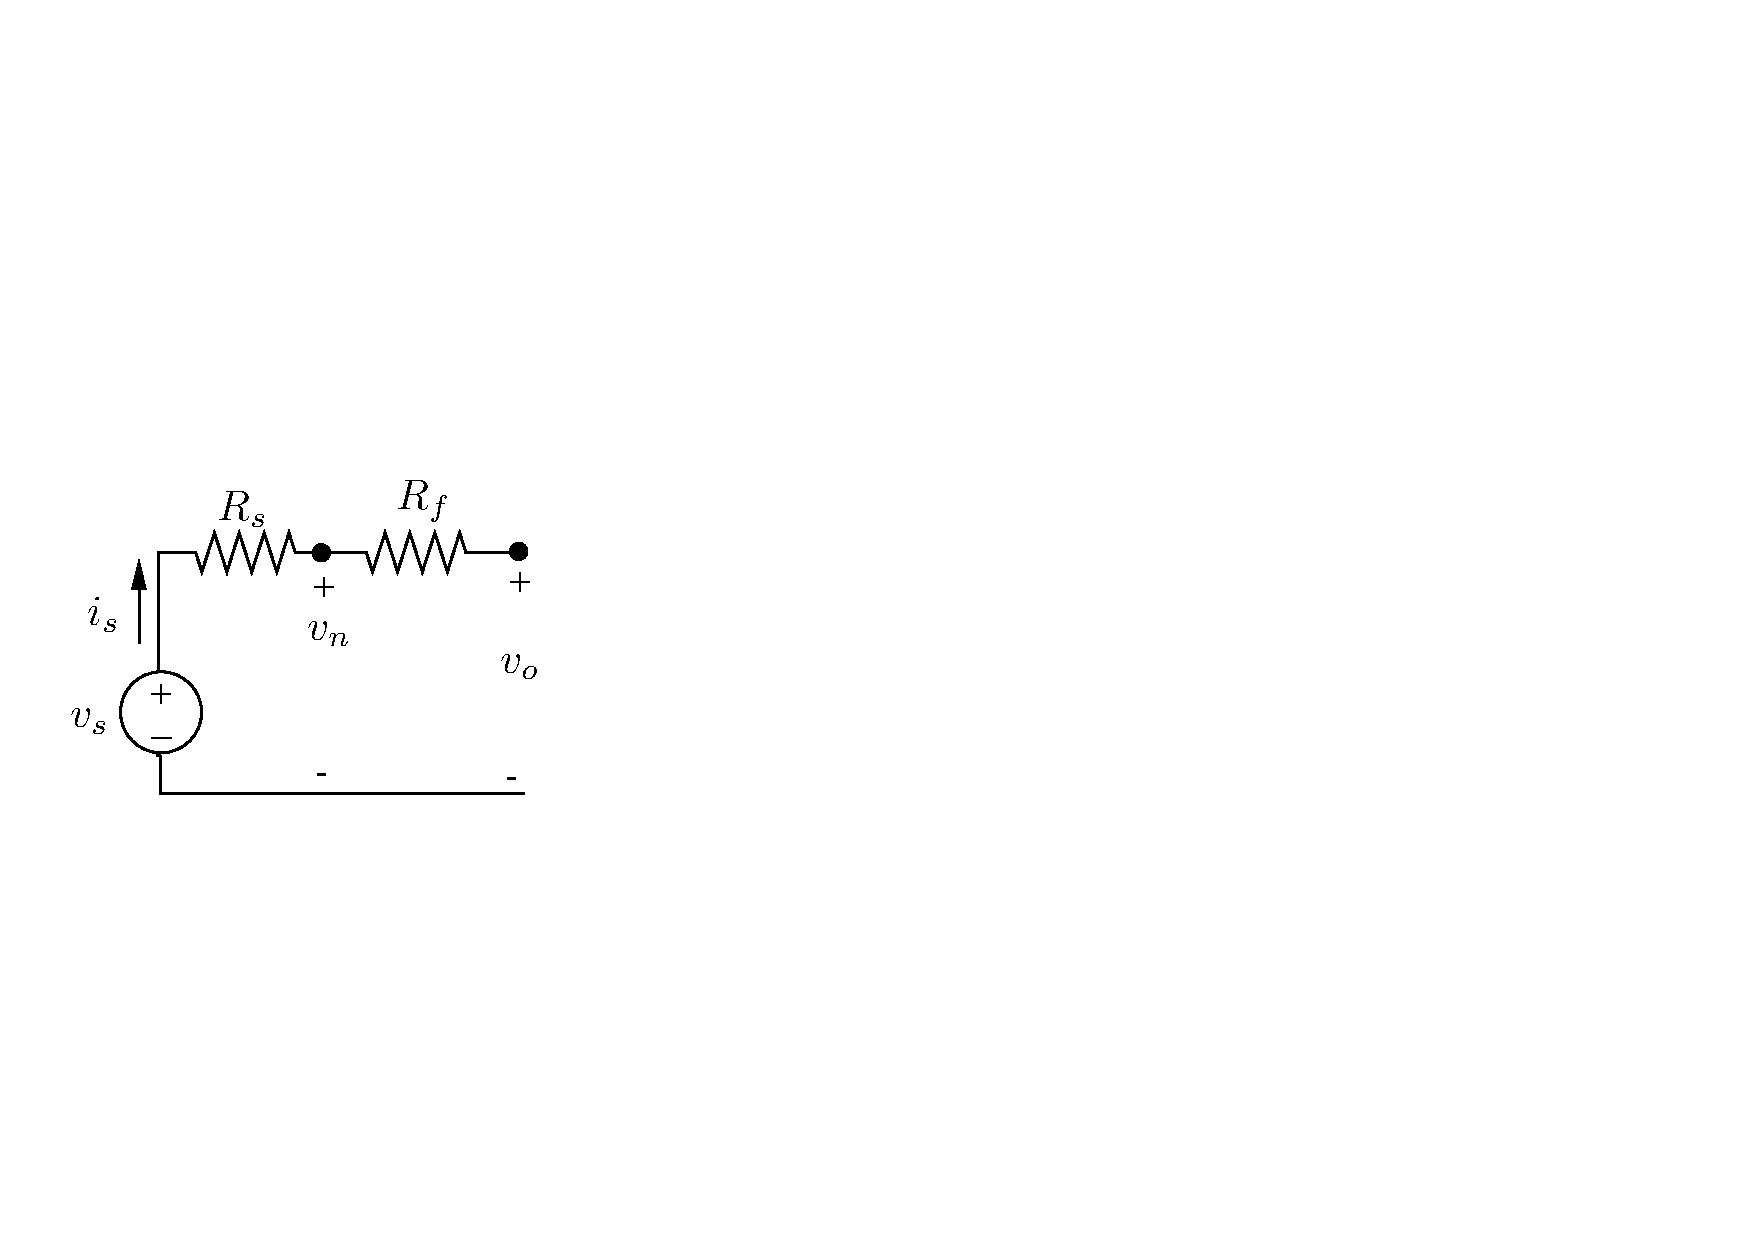
\includegraphics[width=0.9\linewidth]{figs/AO_contre_reaction}
		\end{column}
		\begin{column}{0.5\linewidth}
			En appliquant le théorème de superposition et la formule du diviseur de tension : 
			\[v_n=v_s\frac{R_f}{R_f+R_s}+v_o\frac{R_s}{R_f+R_s}\]
			Taux de contre réaction : $$\frac{ R_s}{R_f+R_s}$$
		\end{column}
	\end{columns}
	
\end{frame}

\begin{frame}{Résistance d'entrée}
	Résistance vue de la source $v_s$ :
	$$\boxed{R_{in}=\frac{v_s}{i_s}=R_s}$$
	
	On souhaite généralement 
	\begin{itemize}
		\item soit que la résistance d'entrée soit la plus grande possible, de manière à ne pas perturber le circuit en amont.
		\item soit quelle soit \textbf{adaptée} au circuit en amont (e.g. en radio) pour maximiser le transfert de puissance.
	\end{itemize}
	

\end{frame}

%-------------------------------------------------------------------

\begin{frame}{Choix de $R_s$ et $R_f$}
	
	Les résultats précédents sont valides seulement si l'AO se trouve dans
	sa plage de fonctionnement linéaire. Pour cela, il faut :
	\[|v_o| < V_{sat},\quad \left|\frac{R_f}{R_s}v_s\right| < V_{sat},
	\quad \frac{R_f}{R_s} < \left|\frac{V_{sat}}{v_s}\right|\]
	
	Exemple :
	\begin{itemize}
		\item $V_{sat}=15$ V
		\item $v_s=10$ mV
		\item $\rightarrow  \frac{R_f}{R_s} < 1500$
	\end{itemize}
\end{frame}

%-------------------------------------------------------------------

\subsection{Circuit intégrateur}
\begin{frame}{Intégrateur}
	
	
	\begin{columns}
		\begin{column}{0.5\linewidth}
			\begin{circuitikz} [scale=1]
				\draw (3.5,1.5) node[op amp] (opamp) {} % Opamp
				(opamp.+) node[left] {$v_p$}
				(opamp.-) node[below] {$v_n$};
				\draw (0,0) coordinate (A) % 
				to[american voltage source, l=$v_s$, i^>=$i_s$, invert] (A |- opamp.-)
				to[R, l=$R_s$, -*] ++(1.5, 0) coordinate(VN);
				\draw (VN) to[short, i=$i_n$, -o] (opamp.-);
				\draw (VN) to[short, i=$i_f$] ++(0,1) coordinate (leftRf)
				to[C, l=\alert{$C$}, color=myRed] (leftRf -| opamp.out) 
				to[short,-*] (opamp.out);
				\draw (opamp.out) to[short, o-o] ++(0.3,0) node[below] {$v_o$};
				\draw (0,0) to[short,-o] ++(5,0);
				\draw (opamp.+) to[short,o-*] (opamp.+ |- A) node[ground]{};
			\end{circuitikz}
		\end{column}
		\begin{column}{0.5\linewidth}
			Plage de fonctionnement linéaire \\ recours aux phaseurs et impédances
			
			\[\frac{\bar{V}_0}{\bar{V}_s}=-\, \frac{Z_f(j\omega)}{Z_s(j\omega)}=-\frac{1}{j\omega R_sC}\]
		\end{column}
	\end{columns}
\end{frame}

%-------------------------------------------------------------------

\subsection{Circuit dérivateur}
\begin{frame}{Dérivateur}
	
	\begin{columns}
		\begin{column}{0.5\linewidth}
			\begin{circuitikz} [scale=1]
				\draw (3.5,1.5) node[op amp] (opamp) {} % Opamp
				(opamp.+) node[left] {$v_p$}
				(opamp.-) node[below] {$v_n$};
				\draw (0,0) coordinate (A) % 
				to[american voltage source, l=$v_s$, i^>=$i_s$, invert] (A |- opamp.-)
				to[C, l=\alert{$C$}, -*, color=myRed] ++(1.5, 0) coordinate(VN);
				\draw (VN) to[short, i=$i_n$, *-o] (opamp.-);
				\draw (VN) to[short, i=$i_f$] ++(0,1) coordinate (leftRf)
				to[R, l=$R_f$] (leftRf -| opamp.out) 
				to[short,-*] (opamp.out);
				\draw (opamp.out) to[short, o-o] ++(0.3,0) node[below] {$v_o$};
				\draw (0,0) to[short,-o] ++(5,0);
				\draw (opamp.+) to[short,o-*] (opamp.+ |- A) node[ground]{};
			\end{circuitikz}
		\end{column}
		\begin{column}{0.5\linewidth}
			Plage de fonctionnement linéaire \\ recours aux phaseurs et impédances
			
			\[\frac{\bar{V}_0}{\bar{V}_s}=- \, \frac{Z_f(j\omega)}{Z_s(j\omega)}=-j\omega R_fC\]
		\end{column}
	\end{columns}
	
\end{frame}

%-------------------------------------------------------------------

\subsection{Circuit source de courant}
\begin{frame}{Source de courant}
	
	\begin{columns}
		\begin{column}{0.5\linewidth}
			\begin{circuitikz} [scale=1]
				\draw (3.5,1.5) node[op amp] (opamp) {} % Opamp
				(opamp.+) node[left] {$v_p$}
				(opamp.-) node[below] {$v_n$};
				\draw (0,0) coordinate (A) % 
				to[american voltage source, l=$v_s$, i^>=\alert{$i$}, invert] (A |- opamp.-)
				to[R, l=$R_s$, -*] ++(1.5, 0) coordinate(VN);
				\draw (VN) to[short, i=$0$, -o] (opamp.-);
				\draw (VN) to[short, i=\alert{$i$}] ++(0,1) coordinate (leftRf)
				to[R, l=\alert{$R_L$}, color=myRed] (leftRf -| opamp.out) 
				to[short,-*] (opamp.out);
				%\draw (opamp.out) to[short, o-o] ++(0.3,0) node[below] {$v_o$};
				%\draw (0,0) to[short,-o] ++(5,0);
				\draw (opamp.+) to[short,o-*] (opamp.+ |- A) node[ground]{} to[short] (A);
			\end{circuitikz}
		\end{column}
		\begin{column}{0.5\linewidth}
			Placer la charge $R_L$ dans la branche de feedback.\\
			Le courant
			\[i=\frac{v_s}{R_s}\]
			est \textbf{indépendant de la charge}.
		\end{column}
	\end{columns}
	
	%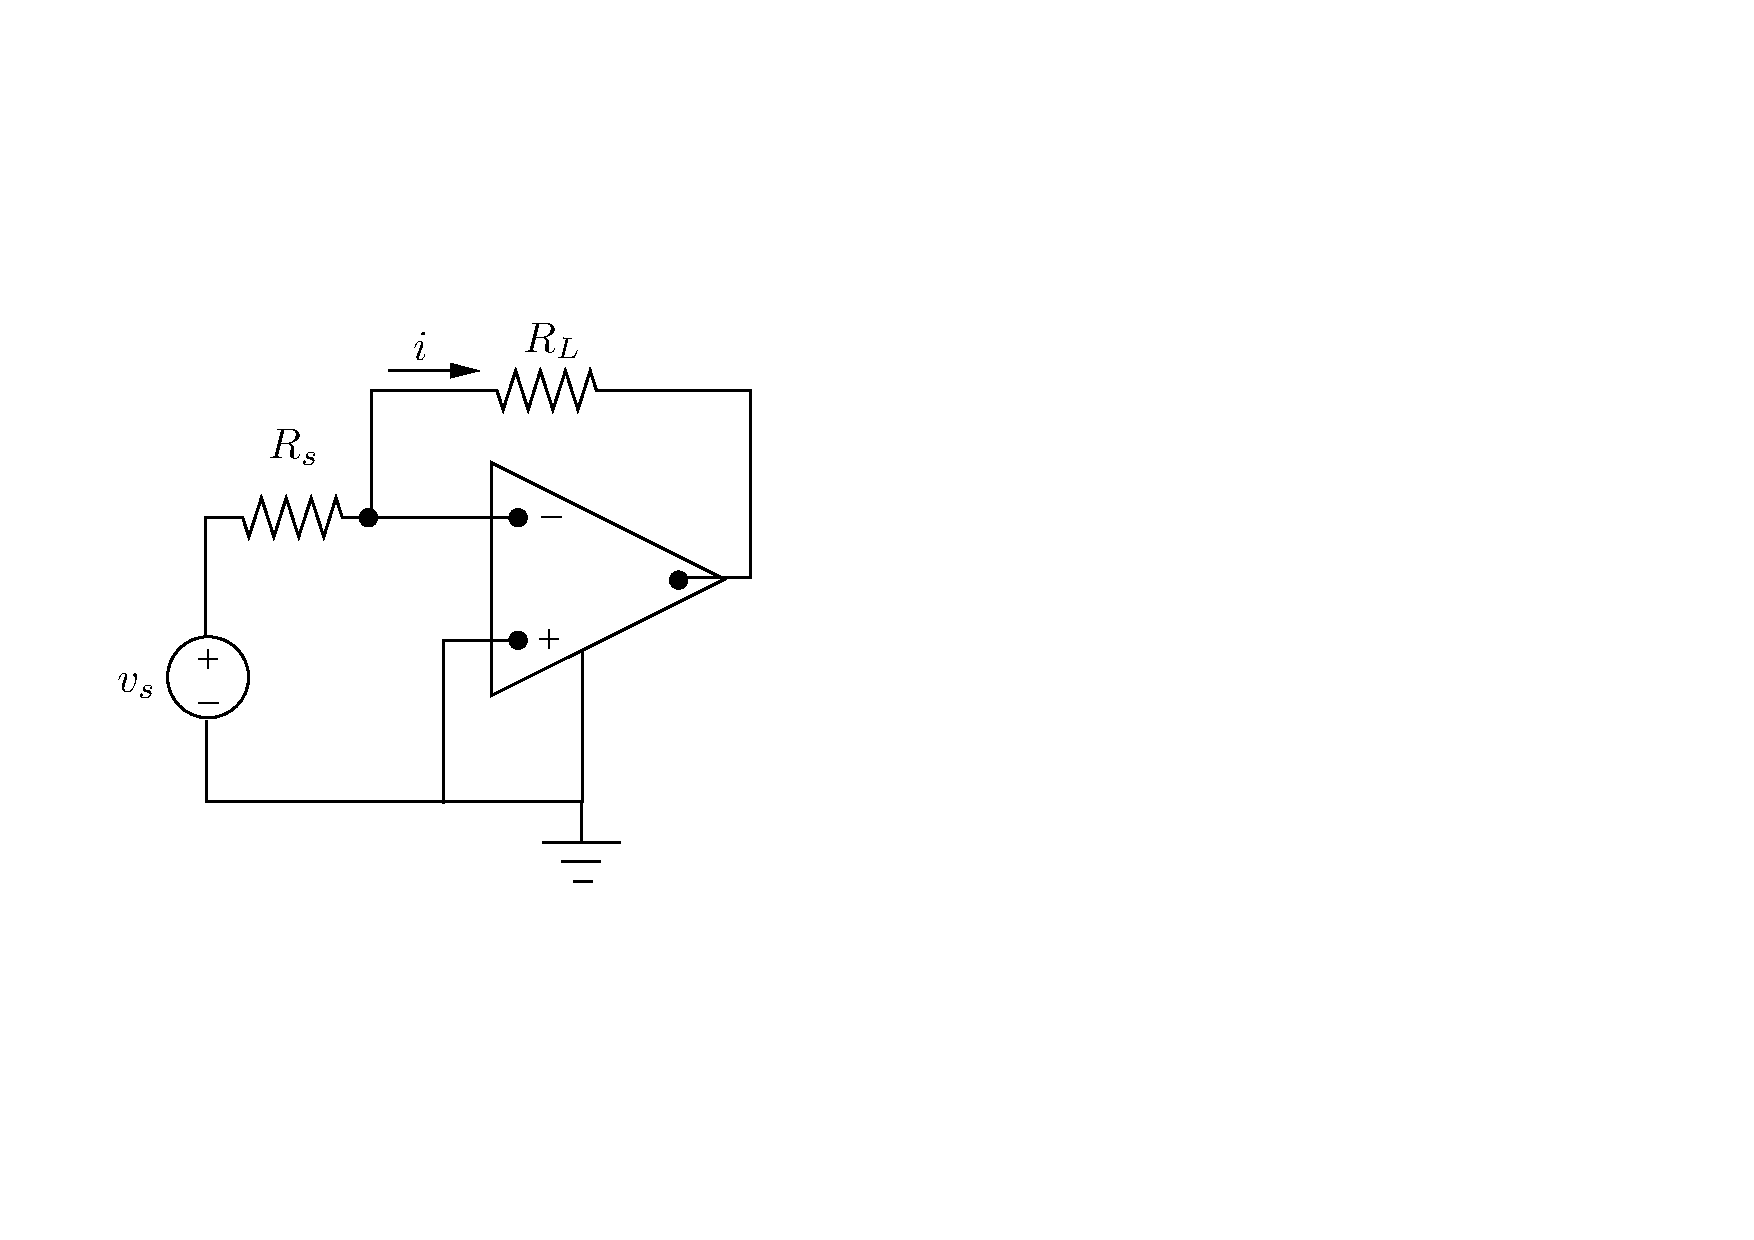
\includegraphics[width=0.6\linewidth]{figs/AO_sourceI}
	
	
\end{frame}


%-------------------------------------------------------------------

\section{Le montage amplificateur non-inverseur}

\subsection{Caractéristiques}

\begin{frame}{Gain en tension}
	
	Hypothèses: AO idéal et fonctionnement linéaire
	
	\begin{columns}
		\begin{column}{0.5\linewidth}
			\begin{center}
				\begin{circuitikz} [scale=1]
					\draw (3.5,2.5) node[op amp] (opamp) {} % Opamp
					(opamp.+) node[below] {$v_p$}
					(opamp.-) node[below] {$v_n$};
					\draw (0,0) coordinate (A) % 
					to[short] (A |- opamp.-)
					to[R, l=$R_s$, -*] ++(1.5, 0) coordinate(VN);
					\draw (VN) to[short, i=$i_n$, -o] (opamp.-);
					\draw (VN) to[short, i=$i_f$] ++(0,1) coordinate (leftRf)
					to[R, l=$R_f$] (leftRf -| opamp.out) 
					to[short,-*] (opamp.out);
					\draw (opamp.out) to[short, o-o] ++(0.3,0) node[below] {$v_o$};
					\draw (A) to[short,-o] ++(5,0);
					\draw (0.7, 0) coordinate (B) node[ground]{} to[american voltage source, l_=$v_g$, i^>=$i_p$, invert] (B |- opamp.+)to[R,l=$R_g$, -o] (opamp.+);
				\end{circuitikz}
			\end{center}
		\end{column}
		\begin{column}{0.4\linewidth}
			\[i_p=0 \, \rightarrow \, v_p=v_g=v_n\]
			\[i_n=0 \, \rightarrow \, v_n=v_g=v_o 
			\frac{R_s}{R_s+R_f}\]
			\begin{center}
				\fbox{$\frac{\displaystyle v_o}{\displaystyle v_g}=\frac{\displaystyle R_f+R_s}{\displaystyle R_s}$}
			\end{center}
		\end{column}
	\end{columns}
\end{frame}


%-------------------------------------------------------------------

\begin{frame}{Caractéristiques du montage}
	\begin{columns}
		\begin{column}{0.4\linewidth}
			Calcul du taux de contre-réaction :
			\[v_n=v_o\frac{R_s}{R_f+R_s}\]
			Taux de contre réaction : $\frac{R_s}{R_f+R_s}$
		\end{column}
		\begin{column}{0.5\linewidth}
			\begin{center}
				\begin{circuitikz}
					\draw (0,0) coordinate (A) 
					to [short] ++(0,2)
					to [R, l=$R_s$, -*] ++ (1.5,0) coordinate (VN)
					to [R, l=$R_f$, -o] ++ (1.5,0) coordinate (VO);
					\draw (A) node[ground] {} to[short, -o] ++(3,0);
					\draw (VN) node[below]{$v_n$};
					\draw (VO) node[below]{$v_o$};
				\end{circuitikz}
			\end{center}
		\end{column}
	\end{columns}
	
	La \textbf{résistance d'entrée} est la résistance vue de la source $v_g$ : $i_p=0 \rightarrow \boxed{R_{in}=\infty}$


	Le montage fonctionne dans la plage linéaire si :
	\[\frac{R_s+R_f}{R_s} < \left|\frac{V_{sat}}{v_g}\right|\]
	
	Cela guide le choix pour $R_s$ et $R_f$

\end{frame}
%-------------------------------------------------------------------

\subsection{Circuit isolateur ou suiveur}
\begin{frame}{Isolateur ou suiveur (voltage follower)}
	
	\begin{columns}
		\begin{column}{0.5\linewidth}
			\begin{circuitikz} [voltage dir=EF, scale=1]
				\draw (3.5,2.5) node[op amp] (opamp) {} % Opamp
				(opamp.+) node[below] {$v_p$}
				(opamp.-) node[below] {$v_n$};
				\draw (0,0) coordinate (A) % 
				to[open] (A |- opamp.-);
				\draw (opamp.-) to[short] ++(-1, 0) coordinate(VN);
				%\draw (VN) to[short, i=$i_n$, -o] (opamp.-);
				\draw (VN) to[short] ++(0,1) coordinate (leftRf)
				to[short] (leftRf -| opamp.out) 
				to[short,-*] (opamp.out);
				\draw (opamp.out) to[short, o-o] ++(0.3,0) node[below] {$v_o$};
				\draw (0.7, 0) coordinate (B) node[ground]{}
				to[american voltage source, l_=$v_g$, i^>=$0$, invert] (B |- opamp.+)to[R,l=$R_g$, -o] (opamp.+);
				\draw (B) to[short] (B -| opamp.out) to[short,-o] ++(0.3,0);
			\end{circuitikz}
			%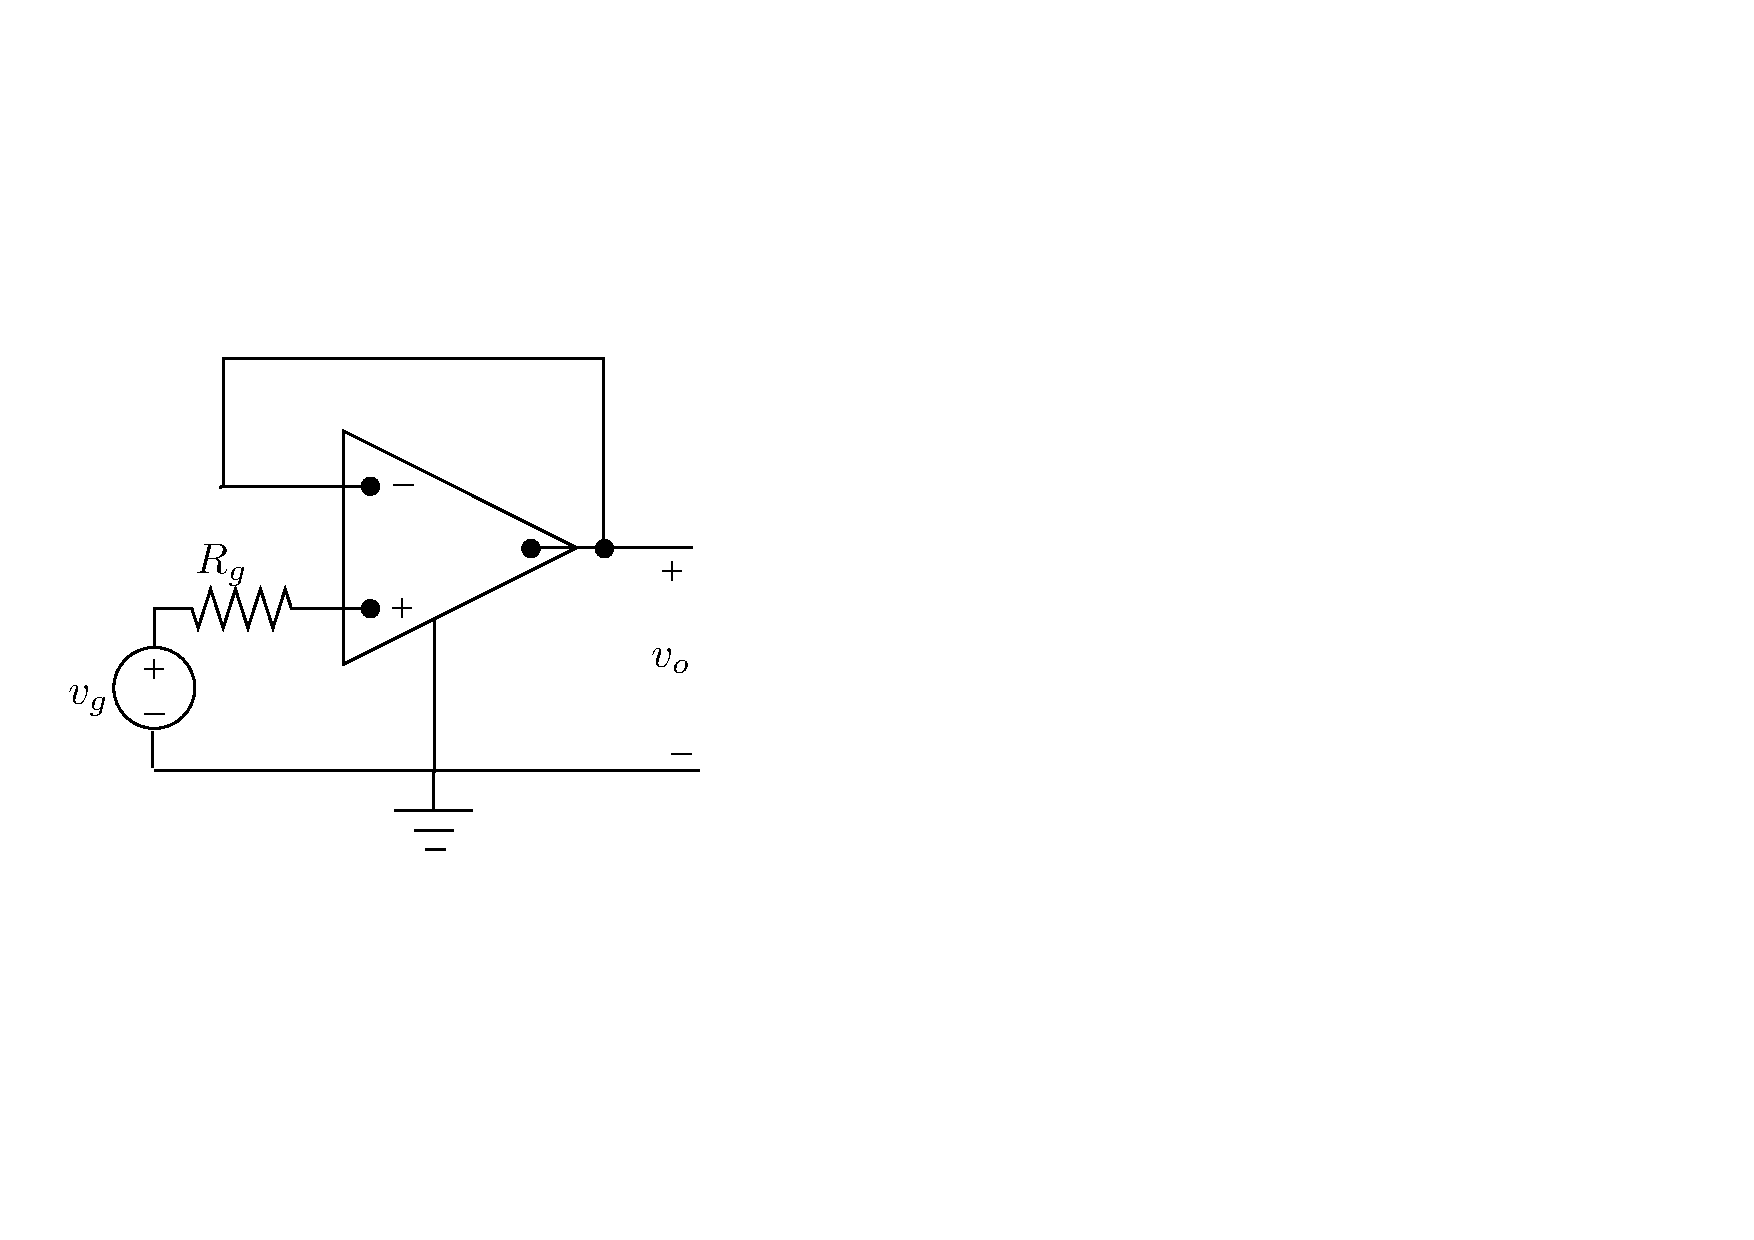
\includegraphics[width=0.8\linewidth]{figs/AO_suiveur}
		\end{column}
		\begin{column}{0.5\linewidth}
			\[v_o=v_g\]
			Vu de la charge, tout se passe comme si la source de tension était
			idéale\\
			$v_o=v_g$ indépendamment de la résistance de charge
		\end{column}
	\end{columns}
	\begin{center}
		Ce montage permet d'isoler deux parties de circuit.
	\end{center}
\end{frame}

%-------------------------------------------------------------------

\section{Addition et soustraction}
\begin{frame}{Additionneur}
	\begin{columns}
		\begin{column}{0.6\linewidth}
			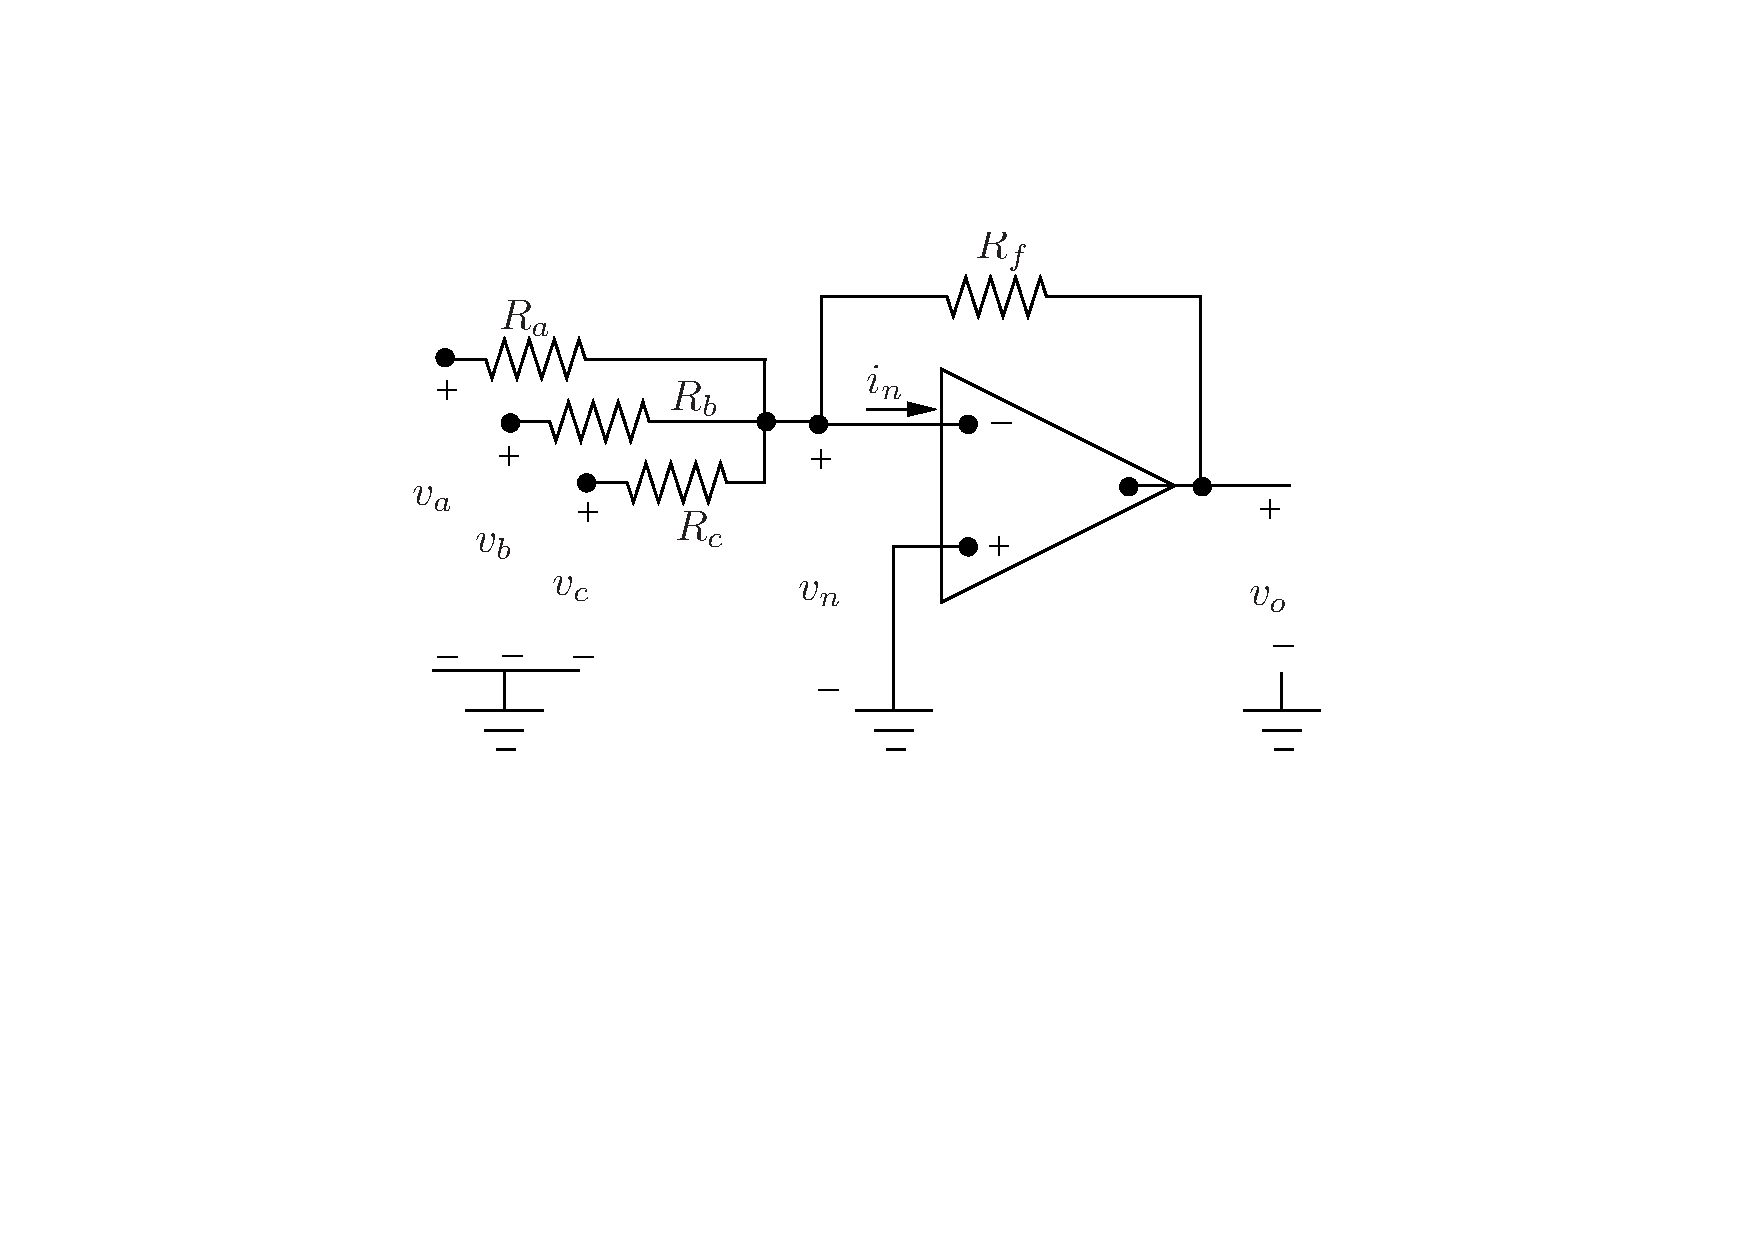
\includegraphics[width=01\linewidth]{figs/AO_add}
		\end{column}
		\begin{column}{0.4\linewidth}
			Par application du théorème de superposition (on suppose toujours
			se trouver dans la plage de fonctionnement linéaire de l'AO)
			$$\boxed{v_o=-\left(\frac{R_f}{R_a}v_a+\frac{R_f}{R_b}v_b+\frac{R_f}{R_c}v_c\right)}$$
		\end{column}
	\end{columns}
\end{frame}
%-------------------------------------------------------------------

\begin{frame}{Soustracteur}
	
	\begin{columns}
		\begin{column}{0.6\linewidth}
			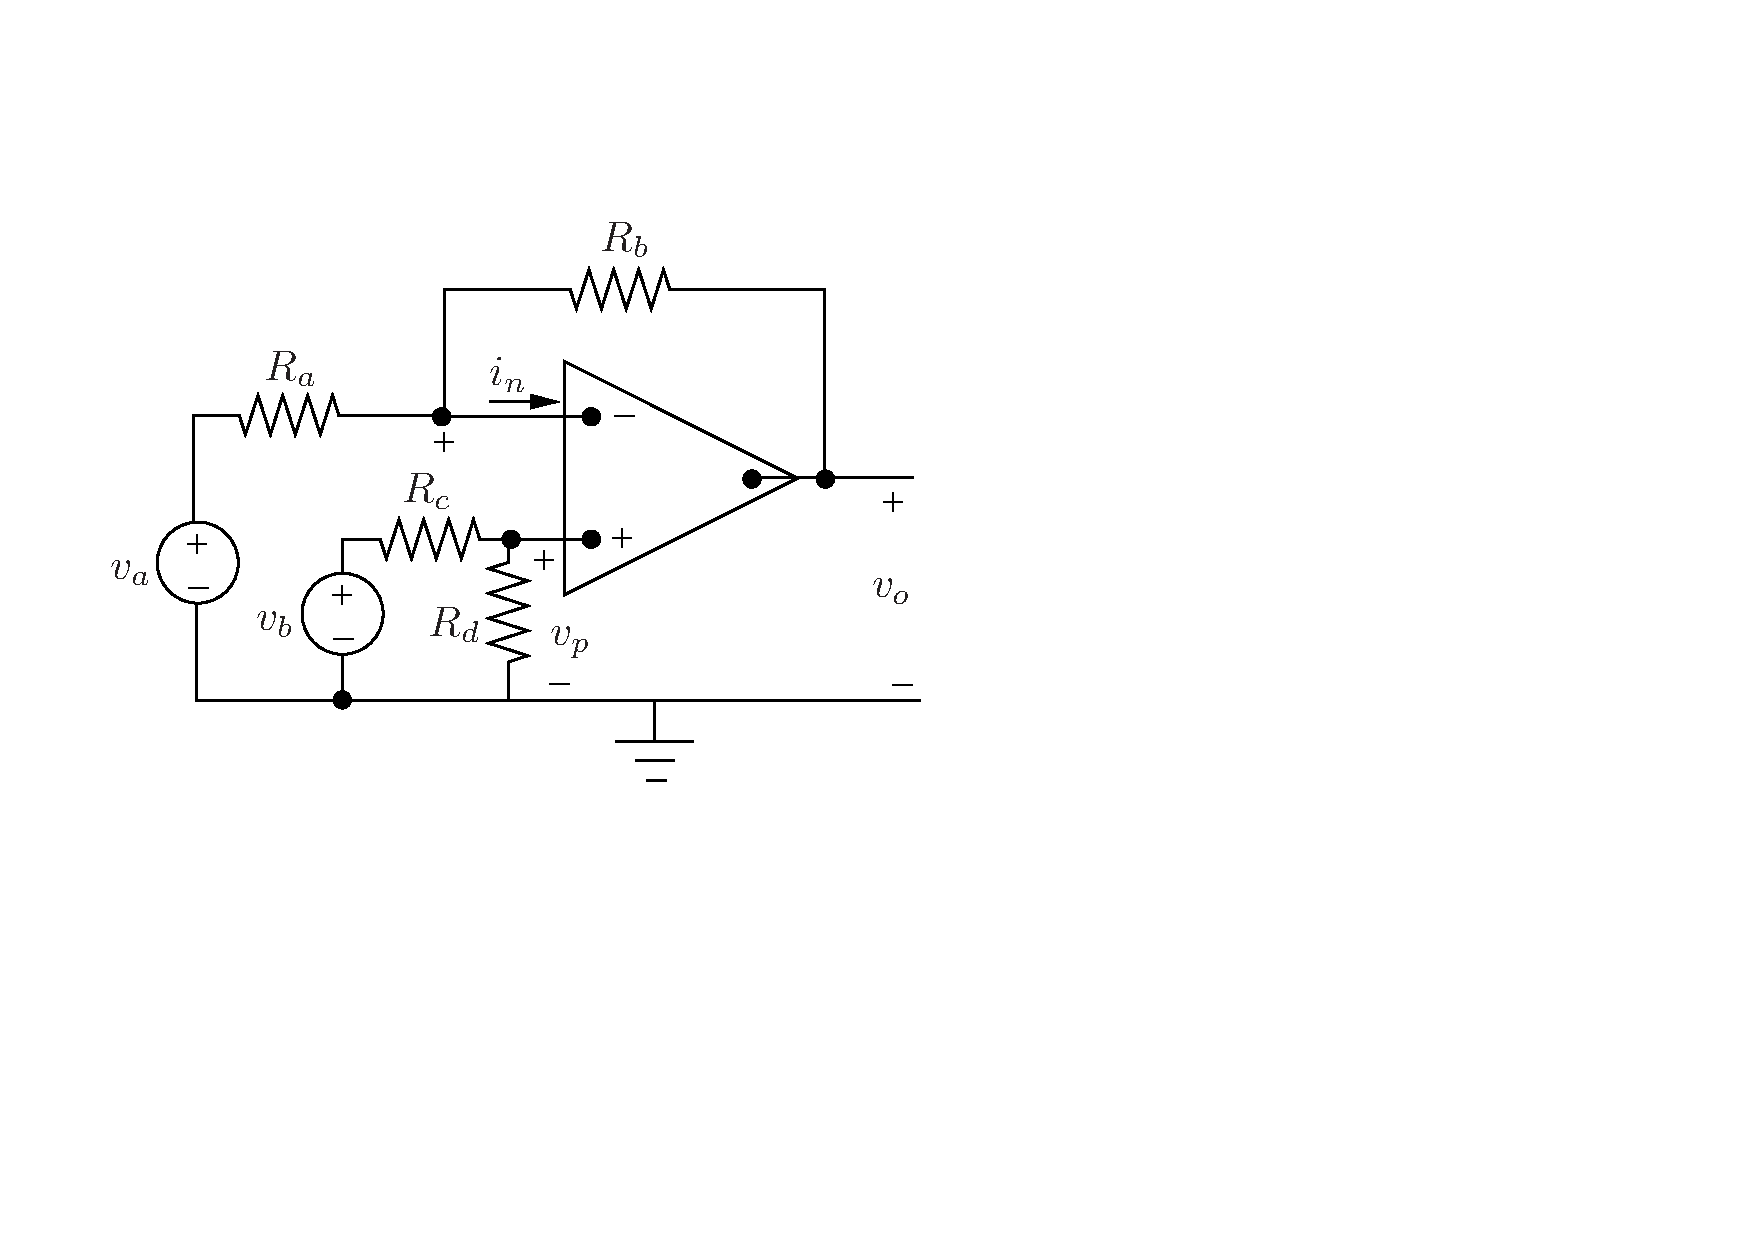
\includegraphics[width=0.9\linewidth]{figs/AO_sub}
		\end{column}
		\begin{column}{0.4\linewidth}
			Par application du théorème de superposition : 
			1. $v_a$ agit seule : montage inverseur
			\[v_o^a=-\frac{R_b}{R_a}v_a\]
			2. $v_b$ agit seule : montage non inverseur
			\[v_o^b=(\frac{R_a+R_b}{R_a})(\frac{R_d}{R_c+R_d})v_b\]
		\end{column}
	\end{columns}
	
	Finalement
	$$\boxed{v_o=(\frac{R_a+R_b}{R_a})(\frac{R_d}{R_c+R_d})v_b-\frac{R_b}{R_a}v_a}$$
\end{frame}

\begin{frame}{Filtre actif}

\begin{columns}
  \begin{column}{0.5\textwidth}
	\begin{center}
		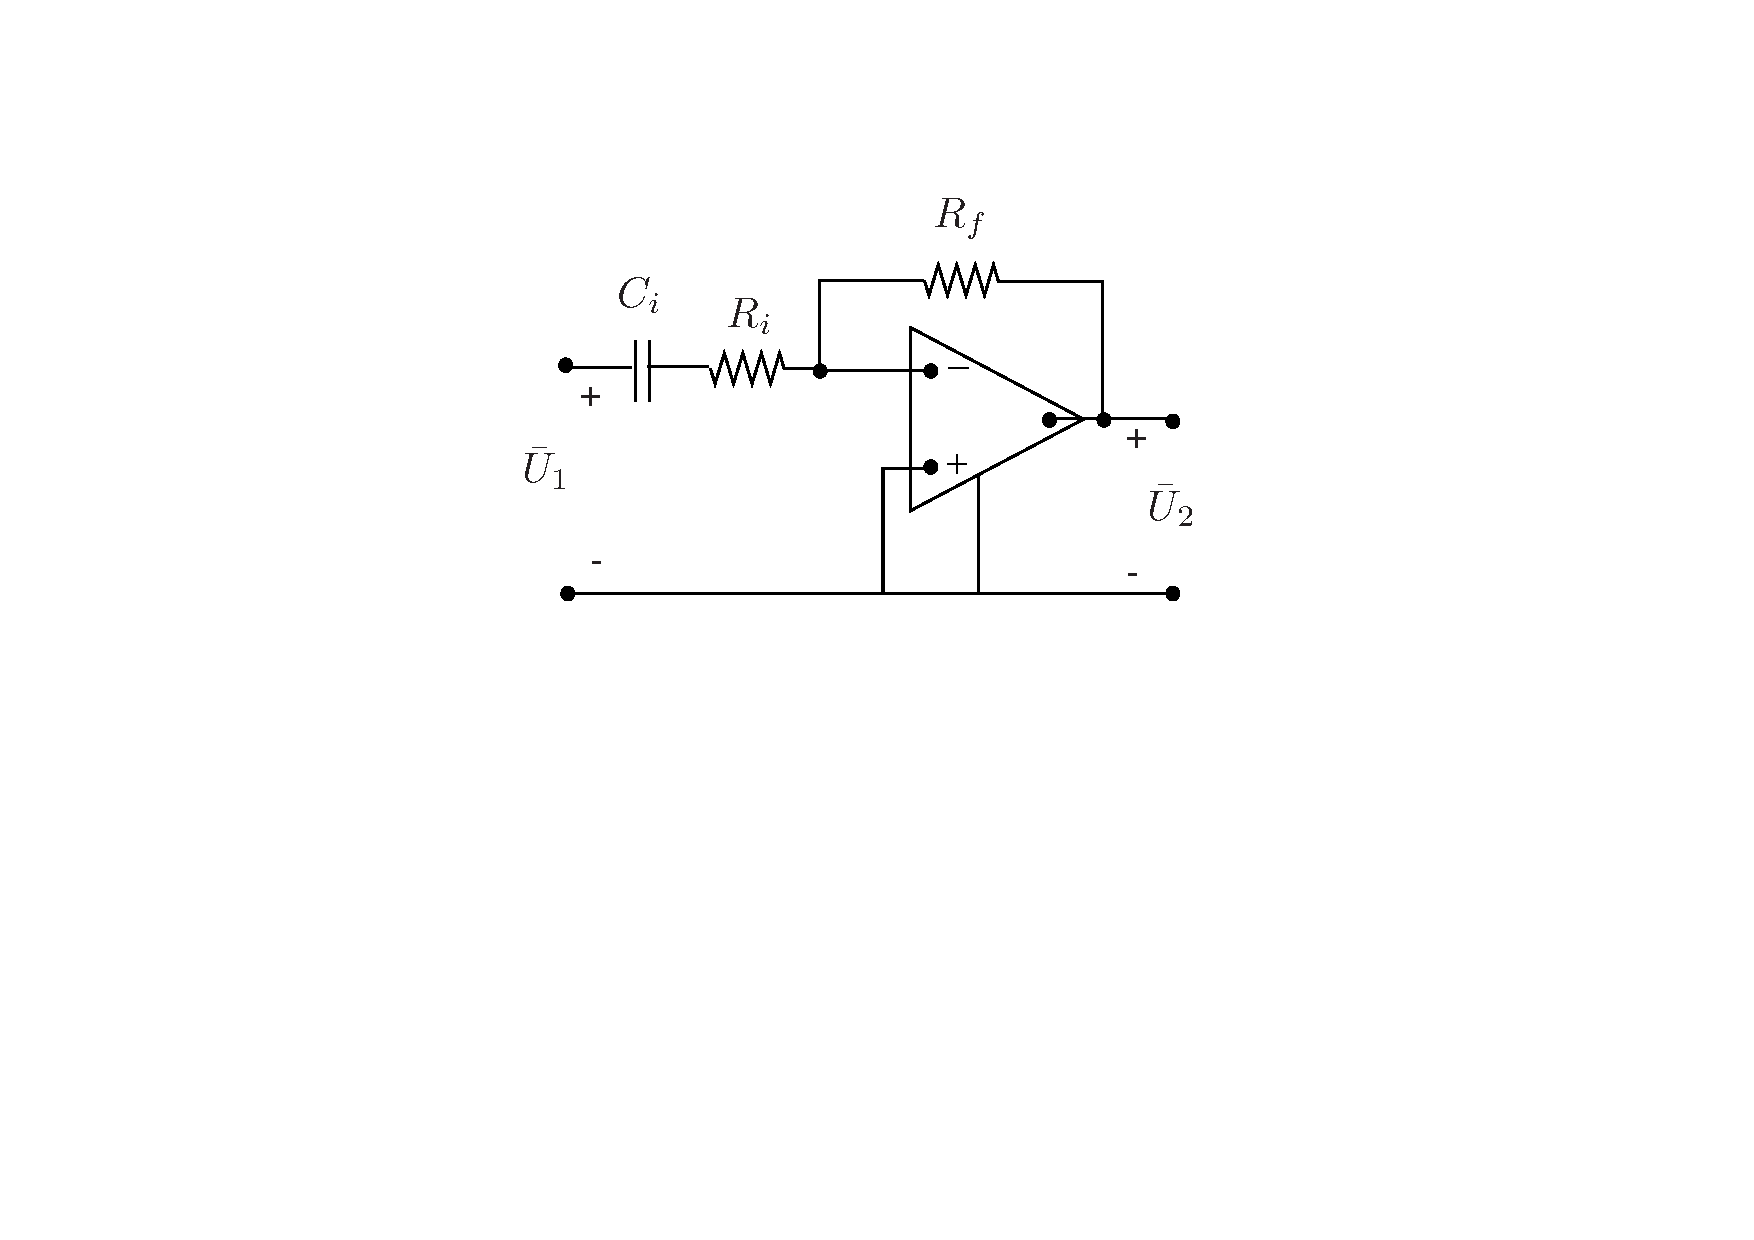
\includegraphics[width=\linewidth]{figs/filtre_actif}
	\end{center}  
  \end{column}
  \begin{column}{0.45\textwidth}
	$$\boxed{H(j\omega)=-\frac{j\omega R_fC_i}{1+j\omega R_iC_i}}$$
	Pulsation de coupure à -3 dB :
	\[\omega_c=\frac{1}{R_iC_i}\]
	\end{column}
\end{columns}
\end{frame}
